\documentclass[12pt]{article}

\usepackage{amsmath}
\usepackage{amssymb}
\usepackage{graphicx}
\usepackage{pifont}
\usepackage{listings}
\usepackage{xcolor}
\usepackage[T1]{fontenc}
\usepackage[utf8]{inputenc}
\usepackage{textcomp}
\usepackage{booktabs}
\usepackage{multirow}

\usepackage{pgf}
\usepackage{tikz}
\usetikzlibrary{arrows,automata}

\definecolor{listinggray}{gray}{0.9}
\definecolor{lbcolor}{rgb}{0.9,0.9,0.9}
\lstset{
	language=C++,
	frame = tb,
	numbers = left,
	showstringspaces = false,
	basicstyle=\ttfamily,
	keywordstyle=\color{blue}\ttfamily,
	stringstyle=\color{red}\ttfamily,
	commentstyle=\color{green}\ttfamily,
	morecomment=[l][\color{magenta}]{\#} 
}

\begin{document}

\begin{titlepage}
	\newcommand{\HRule}{\rule{\linewidth}{0.5mm}}
	
	\center
	
	\textsc{\Large Elektrotehnički fakultet Univerziteta Sarajevo}\\[4cm]
	
	{\huge\bfseries Diskretna Matematika\vspace{5mm}

 	Zadaća 3}\\[4.5cm]

	\begin{minipage}{0.4\textwidth}
		\begin{flushleft}
			\large
			\textit{Student}\\
			Vedad Fejzagić\\[5mm]
			\textit{Broj indeksa}\\
			17336\\[5mm]
			\textit{Grupa}\\
			RI2-2
		\end{flushleft}
	\end{minipage}
	~
	\begin{minipage}{0.4\textwidth}
		\begin{flushright}
			\large
			\textbf{Demonstrator}\\
			\hspace{10mm}Šeila Bečirović
		\end{flushright}
	\end{minipage}
	
	\vfill\vfill\vfill
	
	{\large\today}
	
	\vfill
	
\end{titlepage}


\newpage
\section*{Zadatak 1\label{Z1}}

\underline{Postavka:}

Neki eksperiment može dovesti do tri moguća događaja A1, A2 ili A3 iz skupa događaja X. Ova tri događaja imaju respektivno vjerovatnoće 0.25, 0.5 i 0.25. Rezultati tog eksperimenta nisu dostupni direktno, ali se može izvesti testni eksperiment koji daje događaje B1, B2, B3, B4 ili B5 iz skupa događaja Y, koji su u određenoj vezi sa događajima A1, A2 i A3. Vjerovatnoće da testni eksperiment rezultira događajem Bj, j = 1, 2, 3, 4, 5 ukoliko je izvorni eksperiment rezultirao događajem Ai, i = 1, 2, 3 date su u sljedećoj tabeli: 

\begin{table}[hp]
\centering
\begin{tabular}{|l|l|l|l|l|l|}
\hline
p($B_j$ / $A_i$) & $B_1$  & $B_2$  & $B_3$  & $B_4$  & $B_5$ \\ \hline
$A_1$          & 0.05 & 0.25 & 0.1  & 0.5  & 0.1 \\ \hline
$A_2$          & 0.15 & 0.35 & 0.05 & 0.35 & 0.1 \\ \hline
$A_3$          & 0.5  & 0.05 & 0.15 & 0.1  & 0.2 \\ \hline
\end{tabular}
\end{table}

Odredite entropije skupa izvornih i testnih događaja H(X) i H(Y), uvjetne entropije H(X/Y) i H(Y/X), zajedničku entropiju H(X,Y) te srednju količinu informacije I(X,Y) koju testni događaji nose o izvornim događajima.

\underline{Rješenje:}\\


$$H(X) = - \frac{1}{ln 2} \cdot (0.25 \ln{0.25} + 0.5 \ln{0.5} + 0.25 \ln{0.25}) = 1.5$$

Računamo vrijednosti $p(B_j)$ za $j = 1, 2, 3, 4, 5$:

$$p(B_j) = \sum_{i = 1}^{3} p(A_i) \cdot p(B_j / A_i)$$

Dobijamo:

$$p(B_1) = p(A_1) p(B_1 / A_1) + p(A_2) p(B_1 / A_2) + p(A_3) p(B_1 / A_3) = 0.2125$$
$$p(B_2) = 0.25$$
$$p(B_3) = 0.0875$$
$$p(B_4) = 0.325$$
$$p(B_5) = 0.125$$

$$H(Y) =  - \frac{1}{ln 2} \cdot (0.2125 \ln{0.2125} + 0.25 \ln{0.25} +$$ 
$$+ 0.0875 \ln{0.0875} + 0.325 \ln{0.325}  + 0.125 \ln{0.125}) = 2.178432$$

Sada računamo $p(A_i B_j)$, za $i = 1. 2. 3 ; j = 1, 2, 3, 4, 5$ Rezultati prikazani u vidu tabele:

\begin{table}[hp]
\centering
\begin{tabular}{|l|l|l|l|l|l|}
\hline
p($A_i$ $B_j$) & $B_1$    & $B_2$    & $B_3$    & $B_4$   & $B_5$   \\ \hline
$A_1$          & 0.0125 & 0.0625 & 0.025  & 0.125 & 0.025 \\ \hline
$A_2$          & 0.075  & 0.175  & 0.025  & 0.175 & 0.05  \\ \hline
$A_3$         & 0.125  & 0.0125 & 0.0375 & 0.025 & 0.05  \\ \hline
\end{tabular}
\end{table}

$$H(X, Y) = - \sum_{i = 1}^{3} \sum_{j = 1}^{5} p(A_i B_j) \cdot \log_2 p(A_i B_j)$$
$$H(X, Y) = - \frac{1}{\ln{2}} \sum_{i = 1}^{3} \sum_{j = 1}^{5} p(A_i B_j) \cdot \ln{p(A_i B_j)}$$
$$H(X, Y) = 3.4604$$

$$H(X / Y) = H(X, Y) - H(Y) = 1.27608$$
$$H(Y / X) = H(X, Y) - H(X) = 1.9604$$
$$I(X, Y) = H(X) + H(Y) - H(X, Y) = 0.218$$

\newpage

\section*{Zadatak 2\label{Z2}}

\underline{Postavka:}

Na nekom fakultetu, troškove studija za 22\% studenata plaća država, dok su ostali studenti samofinansirajući. Među studentima koji se školuju o trošku države, 47\% studenata stanuje u studentskom domu, dok među samofinansirajućim studentima 32\% studenata stanuje u studentskom domu. Svi studenti koji stanuju u studentskom domu ujedno posjeduju i iskaznicu za subvencionirani javni prevoz, dok među studentima koji ne stanuju u studentskom domu istu iskaznicu posjeduje i 32\% studenata čiji studij plaća država te 40\% samofinansirajućih studenata.\\

Odredite koliku prosječnu količinu informacije saznanje o tome posjeduje li student iskaznicu za subvencionirani javni prenos ili ne nosi o načinu finansiranja njegovog studija (tj. da li ga finansira država ili troškove snosi sam).

\underline{Rješenje:}\\


\newpage

\section*{Zadatak 3\label{Z3}}

\underline{Postavka:}

Markovljev izvor informacija prvog reda emitira četiri različite poruke a, b, c i d. Ovisno od toga koja je poruka posljednja emitirana, izvor se nalazi u jednom od 4 moguća stanja Sa, Sb, Sc i Sd koja redom odgovaraju emitiranim porukama a, b, c odnosno d. Vjerovatnoće da će izvor emitirati neku od ove 4 poruke ovisno od stanja u kojem se nalazi date su u sljedećoj tablici: 

\begin{table}[hp]
\centering
\begin{tabular}{|l|l|l|l|l|}
\hline
p($x_j$ / $S_i$) & a    & b    & c    & d    \\ \hline
$S_a$           & 0.4  & 0.15 & 0.3  & 0.15 \\ \hline
$S_b$           & 0.4  & 0.4  & 0.1  & 0.1  \\ \hline
$S_c$           & 0.05 & 0.35 & 0.1  & 0.5  \\ \hline
$S_d$           & 0.3  & 0.1  & 0.45 & 0.15 \\ \hline
\end{tabular}
\end{table}

Odredite entropiju i redudansu ovog izvora, zatim entropiju sekvenci dužine 6 te vjerovatnoću pojave sekvence aaabdb.

\underline{Rješenje:}\\

Red izvora je r = 1, izvor modeliramo pomoću 4 stanja:

\begin{center}
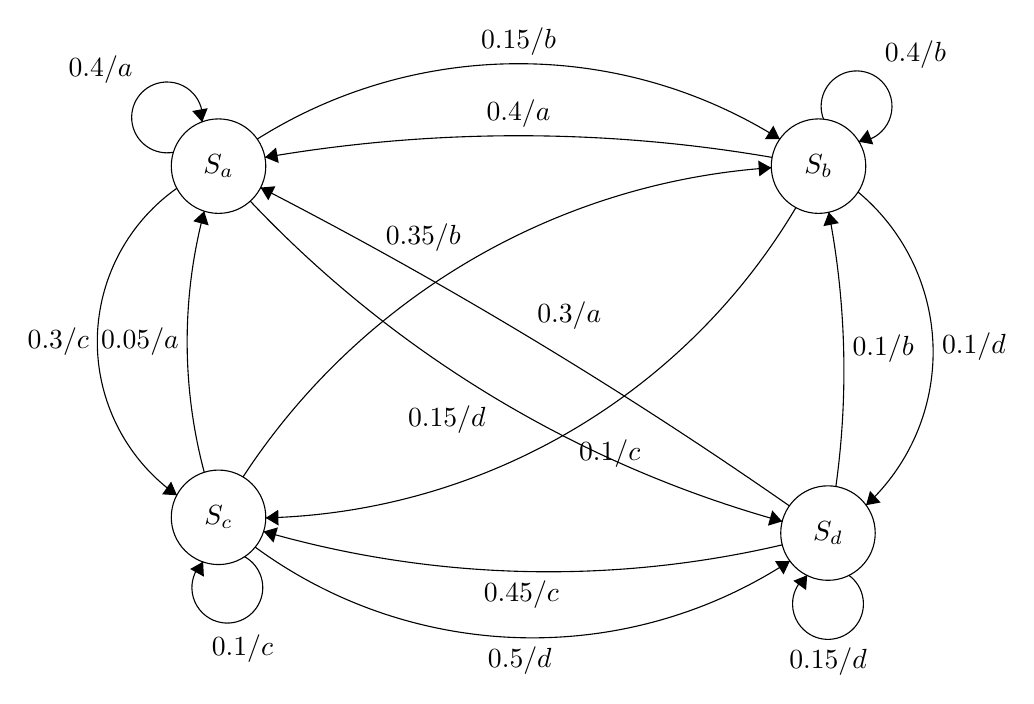
\begin{tikzpicture}[scale=0.2]
\tikzstyle{every node}+=[inner sep=0pt]
\draw [black] (19.5,-16.4) circle (3);
\draw (19.5,-16.4) node {$S_a$};
\draw [black] (57.6,-16.4) circle (3);
\draw (57.6,-16.4) node {$S_b$};
\draw [black] (19.5,-38.7) circle (3);
\draw (19.5,-38.7) node {$S_c$};
\draw [black] (58.2,-39.7) circle (3);
\draw (58.2,-39.7) node {$S_d$};
\draw [black] (21.958,-14.682) arc (122.18765:57.81235:31.147);
\fill [black] (55.14,-14.68) -- (54.73,-13.83) -- (54.2,-14.68);
\draw (38.55,-9.4) node [above] {$0.15/b$};
\draw [black] (22.448,-15.844) arc (99.76857:80.23143:94.903);
\fill [black] (22.45,-15.84) -- (23.32,-16.2) -- (23.15,-15.22);
\draw (38.55,-13.97) node [above] {$0.4/a$};
\draw [black] (16.645,-15.517) arc (280.54816:-7.45184:2.25);
\draw (14.07,-10.29) node [left] {$0.4/a$};
\fill [black] (18.46,-13.6) -- (18.81,-12.72) -- (17.83,-12.9);
\draw [black] (21.145,-41.195) arc (61.12502:-226.87498:2.25);
\draw (21.02,-46.12) node [below] {$0.1/c$};
\fill [black] (18.52,-41.52) -- (17.7,-41.98) -- (18.57,-42.47);
\draw [black] (59.523,-42.38) arc (54:-234:2.25);
\draw (58.2,-46.95) node [below] {$0.15/d$};
\fill [black] (56.88,-42.38) -- (56,-42.73) -- (56.81,-43.32);
\draw [black] (57.923,-13.429) arc (201.52881:-86.47119:2.25);
\draw (63.75,-10.2) node [above] {$0.4/b$};
\fill [black] (60.15,-14.85) -- (61.08,-15.02) -- (60.72,-14.09);
\draw [black] (16.857,-37.297) arc (-125.17132:-234.82868:11.924);
\fill [black] (16.86,-37.3) -- (16.49,-36.43) -- (15.92,-37.24);
\draw (11.3,-27.55) node [left] {$0.3/c$};
\draw [black] (18.593,-35.841) arc (-165.06887:-194.93113:32.18);
\fill [black] (18.59,-19.26) -- (17.9,-19.9) -- (18.87,-20.16);
\draw (17.01,-27.55) node [left] {$0.05/a$};
\draw [black] (55.779,-41.47) arc (-56.71755:-126.24281:29.784);
\fill [black] (55.78,-41.47) -- (54.84,-41.49) -- (55.38,-42.33);
\draw (38.63,-46.91) node [below] {$0.5/d$};
\draw [black] (55.295,-40.449) arc (-76.85012:-106.11025:65.216);
\fill [black] (22.36,-39.6) -- (22.99,-40.3) -- (23.27,-39.34);
\draw (38.73,-42.71) node [below] {$0.45/c$};
\draw [black] (58.251,-19.328) arc (10.91558:-7.96538:53.102);
\fill [black] (58.25,-19.33) -- (57.91,-20.21) -- (58.89,-20.02);
\draw (59.73,-28.01) node [right] {$0.1/b$};
\draw [black] (60.104,-18.04) arc (50.27352:-47.32331:13.224);
\fill [black] (60.62,-37.93) -- (61.54,-37.76) -- (60.87,-37.02);
\draw (65.41,-27.86) node [right] {$0.1/d$};
\draw [black] (55.293,-38.958) arc (-105.49551:-136.60602:73.512);
\fill [black] (55.29,-38.96) -- (54.66,-38.26) -- (54.39,-39.23);
\draw (33.99,-31.6) node [below] {$0.15/d$};
\draw [black] (22.174,-17.759) arc (62.76788:55.13059:294.212);
\fill [black] (22.17,-17.76) -- (22.66,-18.57) -- (23.11,-17.68);
\draw (41.77,-26.8) node [above] {$0.3/a$};
\draw [black] (21.054,-36.135) arc (146.81953:93.8615:43.591);
\fill [black] (54.6,-16.5) -- (53.77,-16.05) -- (53.84,-17.05);
\draw (32.5,-21.87) node [above] {$0.35/b$};
\draw [black] (56.163,-19.033) arc (-30.75497:-88.56399:40.35);
\fill [black] (22.5,-38.74) -- (23.31,-39.22) -- (23.29,-38.22);
\draw (44.34,-33.73) node [below] {$0.1/c$};
\end{tikzpicture}
\end{center}

Računamo vjerovatnoće za svako od stanja rješavanjem sljedećeg sistema jednačina:

$$p(S_a) = p(S_a) p(a/S_a) + p(S_b) p(a/S_b) + p(S_c) p(a/S_c) + p(S_d) p(a/S_d)$$
$$p(S_b) = p(S_a) p(b/S_a) + p(S_b) p(b/S_b) + p(S_c) p(b/S_c) + p(S_d) p(b/S_d)$$
$$p(S_c) = p(S_a) p(c/S_a) + p(S_b) p(c/S_b) + p(S_c) p(c/S_c) + p(S_d) p(c/S_d)$$
$$p(S_a) + p(S_b) + p(S_c) + p(S_d) = 1$$

Nakon uvrštavanja vrijednosti i prebacivanja $p(S_a), p(S_b), p(S_c)$ na desnu stranu jednakosti, dobijamo sljedeću matricu:

\[
M=
  \begin{bmatrix}
    -0.6 & 0.4 & 0.05 & 0.3 & | 0 \\
    0.15 & -0.6 & 0.35 & 0.1 & | 0 \\
	0.3 & 0.1 & -0.9 & 0.45 & | 0 \\
	1 & 1 & 1 & 1 & | 1
  \end{bmatrix}
\]

Koristimo Gausov metod eliminacije da riješimo zadani sistem, svođenjem matrice na desnu trougaonu matricu, dobijamo:

\[
M=
  \begin{bmatrix}
    -0.6	& 0.4	&0.05	&0.3 & | 0 \\
	0 &	-0.5&	0.36&	0.17& |	0\\
	0 &	0	&-0.65&	0.70& |	0\\
	0	&0	&0	&4.54 &| 1
  \end{bmatrix}
\]

$$-0.6p(S_a) + 0.4p(S_b) + 0.05p(S_c) + 0.3p(S_d) = 0$$
$$-0.5p(S_b) + 0.36p(S_c) + 0.17p(S_d) = 0$$
$$-0.65p(S_c) + 0.70p(S_d) = 0$$
$$ 4.54p(S_d) = 1$$
 
Dakle, rješenja sistema su:

$$p(S_a) = 0.29$$
$$p(S_b) = 0.25$$
$$p(S_c) = 0.23$$
$$p(S_d) = 0.22$$


$$H(S_a) = - \frac{1}{\ln{2}} (p(a/S_a) \ln{p(a/S_a)} + p(b/S_a) \ln{p(b/S_a)} + p(c/S_a) \ln{p(c/S_a)} + p(d/S_a) \ln{p(d/S_a)})$$

Analogno za ostale, dobijamo: 

$$H(S_a) \approx 1.871$$
$$H(S_b) \approx 1.722$$
$$H(S_c) \approx 1.578$$
$$H(S_d) \approx 1.782$$

$$H(X/X^{\infty}) = \sum_{i = 1}^{4} p(S_i) H(S_i) = 1.73$$
$$H_{max} = \log_{2}4 = \frac{\ln{4}}{\ln{2}} = 2$$

$$R = \frac{H_{max} - H(X/X^{\infty})}{H_{max}} \approx 0.135 = 13.5\%$$

$$H(X) = - \frac{1}{\ln{2}} (p(a) \ln{p(a)} + p(b) \ln{p(b)} + p(c) \ln{p(c)} + p(d) \ln{p(d)}) \approx 1.98614$$

$$H(X^6) = H(X) + (6 - 1) H(X / X^{\infty}) \approx 10.636$$

$$p(aaabdb) = p(a) p(a/a) p(a/a) p(b/a) p(d/b) p(b/d) = 0.0000696 = 0.00696\%$$


\newpage

\section*{Zadatak 4\label{Z4}}

\underline{Postavka:}

Markovljev izvor informacija drugog reda emitira dvije različite poruke 0 i 1. Ovisno od toga koje su dvije poruke posljednje emitirane, izvor se može naći u jednom od 4 moguća stanja S00, S01, S10 odnosno S11 (recimo, ukoliko su posljednje dvije emitirane poruke 0 i 1 tim redom, izvor će se nalaziti u stanju S01). Vjerovatnoće emitiranja poruke 0 u svakom od tih stanja iznose:

$$p(0/S_{00}) = 0.9$$
$$p(0/S_{01}) = 0.7$$
$$p(0/S_{10}) = 0.1$$
$$p(0/S_{11}) = 0.2$$

Odredite entropiju i redudansu ovog izvora, zatim entropiju sekvenci dužine 6 te vjerovatnoću pojave sekvence 00101100.

\underline{Rješenje:}\\

$$p(0/S_{00}) = 0.9, p(1/S_{00}) = 0.1$$

$$p(0/S_{01}) = 0.7, p(1/S_{01}) = 0.3$$

$$p(0/S_{10}) = 0.1, p(1/S_{10}) = 0.9$$

$$p(0/S_{11}) = 0.2, p(1/S_{11}) = 0.8$$\\

Neka su $S_{00} = S_1$, $S_{01} = S_2$, $S_{10} = S_3$, $S_{11} = S_4$.

\begin{center}
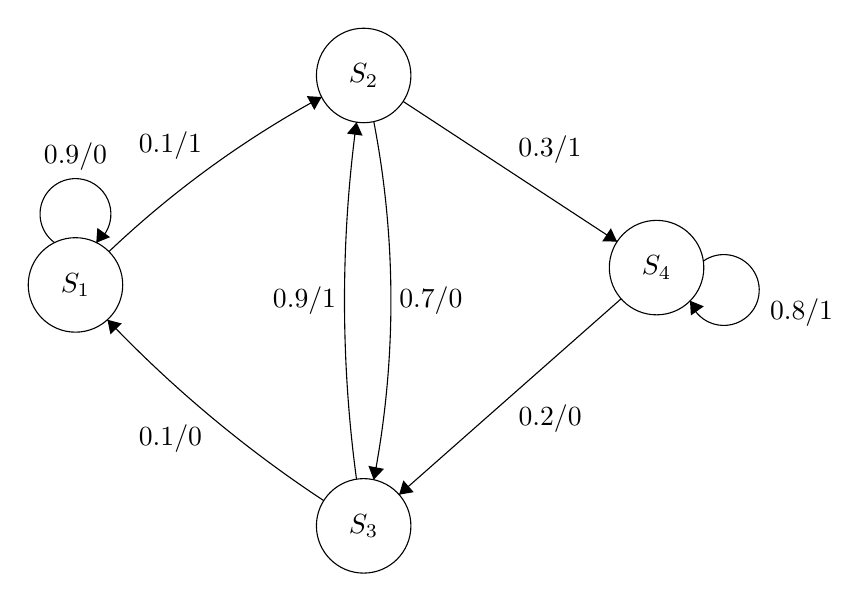
\begin{tikzpicture}[scale=0.2]
\tikzstyle{every node}+=[inner sep=0pt]
\draw [black] (22,-26.9) circle (3);
\draw (22,-26.9) node {$S_1$};
\draw [black] (58.9,-25.8) circle (3);
\draw (58.9,-25.8) node {$S_4$};
\draw [black] (40.3,-13.6) circle (3);
\draw (40.3,-13.6) node {$S_2$};
\draw [black] (40.3,-42.2) circle (3);
\draw (40.3,-42.2) node {$S_3$};
\draw [black] (20.677,-24.22) arc (234:-54:2.25);
\draw (22,-19.65) node [above] {$0.9/0$};
\fill [black] (23.32,-24.22) -- (24.2,-23.87) -- (23.39,-23.28);
\draw [black] (24.126,-24.784) arc (133.5123:118.50521:63.921);
\fill [black] (37.63,-14.97) -- (36.69,-14.91) -- (37.17,-15.79);
\draw (28.03,-18.94) node [above] {$0.1/1$};
\draw [black] (37.765,-40.597) arc (-123.39807:-136.3976:79.091);
\fill [black] (24.03,-29.11) -- (24.22,-30.04) -- (24.94,-29.35);
\draw (28.03,-35.74) node [below] {$0.1/0$};
\draw [black] (39.845,-39.235) arc (-172.30061:-187.69939:84.603);
\fill [black] (39.85,-16.57) -- (39.24,-17.29) -- (40.23,-17.42);
\draw (38.58,-27.9) node [left] {$0.9/1$};
\draw [black] (40.943,-16.53) arc (10.94937:-10.94937:59.861);
\fill [black] (40.94,-39.27) -- (41.59,-38.58) -- (40.6,-38.39);
\draw (42.53,-27.9) node [right] {$0.7/0$};
\draw [black] (42.81,-15.25) -- (56.39,-24.15);
\fill [black] (56.39,-24.15) -- (56,-23.3) -- (55.45,-24.13);
\draw (52.13,-19.2) node [above] {$0.3/1$};
\draw [black] (56.65,-27.78) -- (42.55,-40.22);
\fill [black] (42.55,-40.22) -- (43.48,-40.06) -- (42.82,-39.31);
\draw (52.14,-34.49) node [below] {$0.2/0$};
\draw [black] (61.86,-25.393) arc (125.56505:-162.43495:2.25);
\draw (66.07,-28.64) node [right] {$0.8/1$};
\fill [black] (61.02,-27.9) -- (61.08,-28.84) -- (61.9,-28.26);
\end{tikzpicture}
\end{center}


Potrebne su nam vrijednosti $p(S_1), p(S_2), p(S_3), p(S_4)$

$$p(S_1) = p(S_1) p(0/S_1) + p(S_3) p(0/S_3)$$
$$0.1 p(S_1) = 0.1 p(S_3)$$
$$p(S_1) = p(S_3)$$

Analogno za ostale, dobije se:

$$p(S_2) = p(S_3)$$
$$0.3 p(S_3) = 0.2 p(S_4)$$

Potrebno je riješiti sljedeći sistem:
$$p(S_1) = p(S_3)$$
$$p(S_2) = p(S_3)$$
$$0.3 p(S_3) = 0.2 p(S_4)$$
$$p(S_1) + p(S_2)  + p(S_3) + p(S_4) = 1$$

Rješavanjem sistema, dobiju se sljedeće vrijednosti:

$$p(S_1) = 0.2222$$
$$p(S_2) = 0.2222$$
$$p(S_3) = 0.2222$$
$$p(S_4) = 0.3333$$

$$H(S_1) = - \frac{1}{\ln{2}} (p(0/S_1) \ln{p(0/S_1)} + p(1/S_1) \ln{p(1/S_1)}) \approx 0.47$$
$$H(S_2) \approx 0.881291$$
$$H(S_3) \approx 0.468996$$
$$H(S_4) \approx 0.721928$$

$$H(X/X^{\infty}) = \sum_{i = 1}^{4} p(S_i) H(S_i) = 0.638$$

Redudansa:

$$H_{max} = \log_{2}4 = 2$$
$$R = \frac{H_{max} - H(X/X^{\infty})}{H_{max}} \approx 0.681 \approx 68.1 \%$$ \\

Entropija sekvenci dužine 6:

$$H(X^2) = - \frac{1}{\ln{2}} (p(00) \ln{p(00)} + p(01) \ln{p(01)} + p(10) \ln{p(10)} + p(11) \ln{p(11)}) = 1.96954$$

$$H(X^6) = H(X^2) + 4  H(X/X^{\infty}) \approx 4.52154$$\\

Vjerovatnoća pojave sekvence 00101100:

$$p(00101100) = p(00) p(1/00)p(0/01)p(1/10)p(1/01)p(0/11)p(0/10) = 0.00008316 = 0.008316\%$$


\newpage

\section*{Zadatak 5\label{Z5}}

\underline{Postavka:}

Ergodični izvor informacija bez memorije emitira 10 poruka A, B, C, D, E, F, G, H, I i J. Proučavanjem sekvence dužine 645 koju je emitirao ovaj izvor, uočena je sljedeća učestalost pojavljivanja pojedinih poruka: 

\begin{table}[hp]
\centering
\begin{tabular}{|l|l|l|l|l|l|l|l|l|l|l|}
\hline
Poruka:     & A  & B  & C  & D  & E  & F  & G  & H  & I  & J  \\ \hline
Učestalost: & 18 & 73 & 87 & 49 & 73 & 99 & 98 & 44 & 80 & 24 \\ \hline
\end{tabular}
\end{table}

Za ovaj izvor informacija formirajte:

a) Binarni Shannon-Fano kod sa simbolima 0 i 1;

b) Binarni Huffmanov kod sa simbolima 0 i 1;

c) Ternarni Huffmanov kod sa simbolima 0, 1 i 2.

Za sva tri načina kodiranja, izračunajte protok informacija kroz komunikacioni kanal, procenat iskorištenja kanala veze, te kodirajte sekvencu poruka BAIBBBJIDJCE.

\underline{Rješenje:}\\

a)\\

Sortiramo:

\begin{table}[hp]
\centering
\begin{tabular}{|l|l|}
\hline
F & 99 \\ \hline
G & 98 \\ \hline
C & 87 \\ \hline
I & 80 \\ \hline
B & 73 \\ \hline
E & 73 \\ \hline
D & 49 \\ \hline
H & 44 \\ \hline
J & 24 \\ \hline
A & 18 \\ \hline
\end{tabular}
\end{table}

Kodiramo pomoću binarnog stabla:

\begin{center}
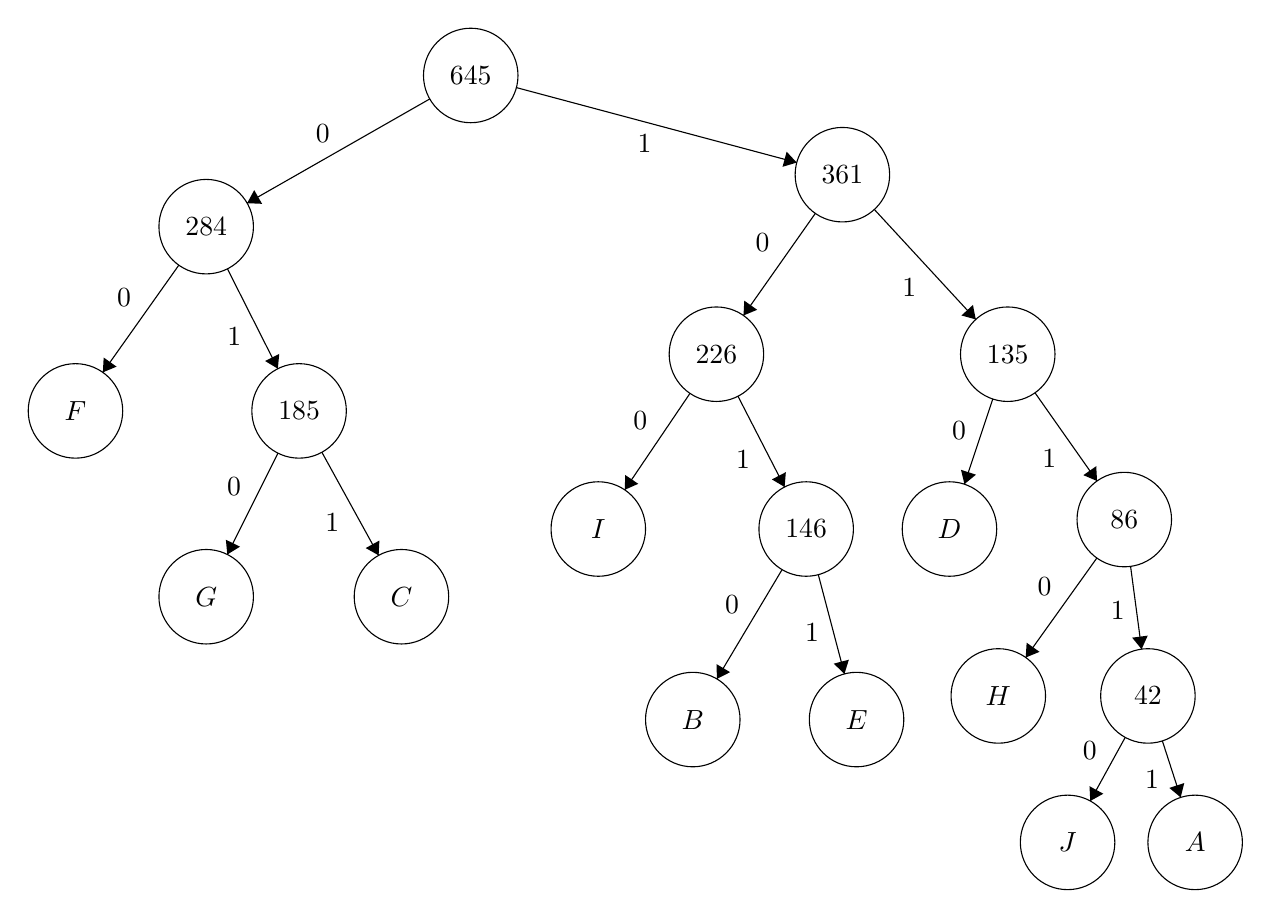
\begin{tikzpicture}[scale=0.2]
\tikzstyle{every node}+=[inner sep=0pt]
\draw [black] (30.9,-5.6) circle (3);
\draw (30.9,-5.6) node {$645$};
\draw [black] (14.1,-15.2) circle (3);
\draw (14.1,-15.2) node {$284$};
\draw [black] (54.5,-11.9) circle (3);
\draw (54.5,-11.9) node {$361$};
\draw [black] (5.8,-26.9) circle (3);
\draw (5.8,-26.9) node {$F$};
\draw [black] (20,-26.9) circle (3);
\draw (20,-26.9) node {$185$};
\draw [black] (14.1,-38.7) circle (3);
\draw (14.1,-38.7) node {$G$};
\draw [black] (26.5,-38.7) circle (3);
\draw (26.5,-38.7) node {$C$};
\draw [black] (46.5,-23.3) circle (3);
\draw (46.5,-23.3) node {$226$};
\draw [black] (65,-23.3) circle (3);
\draw (65,-23.3) node {$135$};
\draw [black] (39,-34.4) circle (3);
\draw (39,-34.4) node {$I$};
\draw [black] (52.2,-34.4) circle (3);
\draw (52.2,-34.4) node {$146$};
\draw [black] (45,-46.5) circle (3);
\draw (45,-46.5) node {$B$};
\draw [black] (55.4,-46.5) circle (3);
\draw (55.4,-46.5) node {$E$};
\draw [black] (61.3,-34.4) circle (3);
\draw (61.3,-34.4) node {$D$};
\draw [black] (72.4,-33.8) circle (3);
\draw (72.4,-33.8) node {$86$};
\draw [black] (64.4,-45) circle (3);
\draw (64.4,-45) node {$H$};
\draw [black] (73.9,-45) circle (3);
\draw (73.9,-45) node {$42$};
\draw [black] (68.8,-54.3) circle (3);
\draw (68.8,-54.3) node {$J$};
\draw [black] (76.9,-54.3) circle (3);
\draw (76.9,-54.3) node {$A$};
\draw [black] (28.3,-7.09) -- (16.7,-13.71);
\fill [black] (16.7,-13.71) -- (17.65,-13.75) -- (17.15,-12.88);
\draw (21.5,-9.9) node [above] {$0$};
\draw [black] (33.8,-6.37) -- (51.6,-11.13);
\fill [black] (51.6,-11.13) -- (50.96,-10.44) -- (50.7,-11.4);
\draw (41.94,-9.31) node [below] {$1$};
\draw [black] (12.36,-17.65) -- (7.54,-24.45);
\fill [black] (7.54,-24.45) -- (8.41,-24.09) -- (7.59,-23.51);
\draw (9.36,-19.68) node [left] {$0$};
\draw [black] (15.45,-17.88) -- (18.65,-24.22);
\fill [black] (18.65,-24.22) -- (18.74,-23.28) -- (17.84,-23.73);
\draw (16.36,-22.16) node [left] {$1$};
\draw [black] (18.66,-29.58) -- (15.44,-36.02);
\fill [black] (15.44,-36.02) -- (16.25,-35.52) -- (15.35,-35.08);
\draw (16.35,-31.69) node [left] {$0$};
\draw [black] (21.45,-29.53) -- (25.05,-36.07);
\fill [black] (25.05,-36.07) -- (25.1,-35.13) -- (24.23,-35.61);
\draw (22.58,-33.99) node [left] {$1$};
\draw [black] (52.78,-14.36) -- (48.22,-20.84);
\fill [black] (48.22,-20.84) -- (49.09,-20.48) -- (48.27,-19.9);
\draw (49.9,-16.24) node [left] {$0$};
\draw [black] (56.53,-14.11) -- (62.97,-21.09);
\fill [black] (62.97,-21.09) -- (62.79,-20.17) -- (62.06,-20.84);
\draw (59.22,-19.06) node [left] {$1$};
\draw [black] (44.82,-25.79) -- (40.68,-31.91);
\fill [black] (40.68,-31.91) -- (41.54,-31.53) -- (40.71,-30.97);
\draw (42.14,-27.51) node [left] {$0$};
\draw [black] (47.87,-25.97) -- (50.83,-31.73);
\fill [black] (50.83,-31.73) -- (50.91,-30.79) -- (50.02,-31.25);
\draw (48.66,-29.98) node [left] {$1$};
\draw [black] (50.67,-36.98) -- (46.53,-43.92);
\fill [black] (46.53,-43.92) -- (47.37,-43.49) -- (46.51,-42.98);
\draw (47.96,-39.19) node [left] {$0$};
\draw [black] (52.97,-37.3) -- (54.63,-43.6);
\fill [black] (54.63,-43.6) -- (54.91,-42.7) -- (53.95,-42.95);
\draw (53.04,-40.95) node [left] {$1$};
\draw [black] (64.05,-26.15) -- (62.25,-31.55);
\fill [black] (62.25,-31.55) -- (62.98,-30.95) -- (62.03,-30.64);
\draw (62.38,-28.15) node [left] {$0$};
\draw [black] (66.73,-25.75) -- (70.67,-31.35);
\fill [black] (70.67,-31.35) -- (70.62,-30.41) -- (69.8,-30.98);
\draw (68.11,-29.92) node [left] {$1$};
\draw [black] (70.66,-36.24) -- (66.14,-42.56);
\fill [black] (66.14,-42.56) -- (67.02,-42.2) -- (66.2,-41.62);
\draw (67.81,-38.03) node [left] {$0$};
\draw [black] (72.8,-36.77) -- (73.5,-42.03);
\fill [black] (73.5,-42.03) -- (73.89,-41.17) -- (72.9,-41.3);
\draw (72.47,-39.55) node [left] {$1$};
\draw [black] (72.46,-47.63) -- (70.24,-51.67);
\fill [black] (70.24,-51.67) -- (71.07,-51.21) -- (70.19,-50.73);
\draw (70.68,-48.46) node [left] {$0$};
\draw [black] (74.82,-47.86) -- (75.98,-51.44);
\fill [black] (75.98,-51.44) -- (76.21,-50.53) -- (75.26,-50.84);
\draw (74.63,-50.32) node [left] {$1$};
\end{tikzpicture}
\end{center}

Kodirane poruke su sljedeće:

\begin{table}[hp]
\centering
\begin{tabular}{|l|l|}
\hline
F & 00    \\ \hline
G & 010   \\ \hline
C & 011   \\ \hline
I & 100   \\ \hline
B & 1010  \\ \hline
E & 1011  \\ \hline
D & 110   \\ \hline
H & 1110  \\ \hline
J & 11110 \\ \hline
A & 11111 \\ \hline
\end{tabular}
\end{table}

Kodirana sekvenca poruka: BAIBBBJIDJCE glasi:

$$10101111110010101010101011110100110111100111011$$

Prosječna dužina kodne riječi: 

$$n_{sr} = \sum_{i = 1}^{10} p_i n_i \approx \sum_{i = 1}^{10} \frac{N_i}{N} n_i = \frac{1}{N} \sum_{i = 1}^{10} N_i n_i$$
$$n_{sr} = 3.271$$

Entropija izvora:

$$H(X/X^{\infty}) = H(X) =  - \sum_{i = 1}^{10} p_i \log_{2}p_i = ... = \frac{1}{\ln{2}} (\ln{N} - \frac{1}{N} \sum_{i = 1}^{10} N_i \ln{N_i})$$
$$H(X/X^{\infty}) = 3.1671$$

Protok informacija:

$$\overline{I(H)} = \frac{H(X/X^{\infty}) }{n_{sr} \tau} \approx \frac{0.968}{\tau}$$

Iskorištenost kanala veze 96.8\%

b)\\

Iz postavke: $n = 10, m = 2 \to m^{*} = 2 + mod(n - 4, m - 1) = 2$
Prelazimo na formiranje binarnog Huffmanovog koda:
\newpage
\begin{table}[hp]
\hspace*{-1.0in}
\begin{tabular}{|l|l|l|l|l|l|l|l|l|l|l|l|l|l|l|l|}
\hline
\multicolumn{2}{|l|}{Početak} & \multicolumn{2}{l|}{Iteracija 1}               & \multicolumn{2}{l|}{Iteracija 2} & \multicolumn{2}{l|}{Iteracija 3} & \multicolumn{2}{l|}{Iteracija 4} & \multicolumn{2}{l|}{Iteracija 5} & \multicolumn{2}{l|}{Iteracija 6} & \multicolumn{2}{l|}{Iteracija 7} \\ \hline
F             & 99            & F   & 99                                       & F       & 99                     & E/0     & \multirow{2}{*}{122}   & I/0     & \multirow{2}{*}{153}   & C/0     & \multirow{4}{*}{173}   & F/0     & \multirow{2}{*}{197}   & I/00    & \multirow{4}{*}{275}   \\ \cline{1-6}
G             & 98            & G   & 98                                       & G       & 98                     & D/1     &                        & B/1     &                        & H/10    &                        & G/1     &                        & B/01    &                        \\ \cline{1-10} \cline{13-14}
C             & 87            & C   & 87                                       & C       & 87                     & F       & 99                     & E/0     & \multirow{2}{*}{122}   & J/110   &                        & C/0     & \multirow{4}{*}{173}   & E/10    &                        \\ \cline{1-8}
I             & 80            & I   & 80                                       & H/0     & \multirow{3}{*}{86}    & G       & 98                     & D/1     &                        & A/111   &                        & H/10    &                        & D/11    &                        \\ \cline{1-4} \cline{7-12} \cline{15-16} 
B             & 73            & B   & 73                                       & J/10    &                        & C       & 87                     & F       & 99                     & I/0     & \multirow{2}{*}{153}   & J/110   &                        & F/0     & \multirow{2}{*}{197}   \\ \cline{1-4} \cline{7-10}
E             & 73            & E   & 73                                       & A/11    &                        & H/0     & \multirow{3}{*}{86}    & G       & 98                     & B/1     &                        & A/111   &                        & G/1     &                        \\ \cline{1-6} \cline{9-16} 
D             & 49            & D   & 49                                       & I       & 80                     & J/10    &                        & C       & 87                     & E/0     & \multirow{2}{*}{122}   & I/0     & \multirow{2}{*}{153}   & C/0     & \multirow{4}{*}{173}   \\ \cline{1-6} \cline{9-10}
H             & 44            & H   & 44                                       & B       & 73                     & A/11    &                        & H/0     & \multirow{3}{*}{86}    & D/1     &                        & B/1     &                        & H/10    &                        \\ \cline{1-8} \cline{11-14}
J             & 24            & J/0 & \multicolumn{1}{c|}{\multirow{2}{*}{42}} & E       & 73                     & I       & 80                     & J/10    &                        & F       & 99                     & E/0     & \multirow{2}{*}{122}   & J/110   &                        \\ \cline{1-2} \cline{5-8} \cline{11-12}
A             & 18            & A/1 & \multicolumn{1}{c|}{}                    & D       & 49                     & B       & 73                     & A/11    &                        & G       & 98                     & D/1     &                        & A/111   &                        \\ \hline
\end{tabular}
\end{table}

\begin{table}[hp]
\centering
\begin{tabular}{|l|l|l|l|}
\hline
\multicolumn{2}{|l|}{Iteracija 8} & \multicolumn{2}{l|}{Iteracija 9} \\ \hline
F/00 & \multirow{6}{*}{370} & I/000 & \multirow{10}{*}{645} \\
G/01 &  & G/001 &  \\
C/10 &  & C/010 &  \\
H/110 &  & H/0110 &  \\
J/1110 &  & J/01110 &  \\
A/1111 &  & A/01111 &  \\ \cline{1-2}
I/00 & \multirow{4}{*}{275} & I/100 &  \\
B/01 &  & B/101 &  \\
E/10 &  & E/110 &  \\
D/11 &  & D/111 &  \\ \hline
\end{tabular}
\end{table}

\textit{U sljedecim zadacima koji zahtjevaju veci broj iteracija, nece citav postupak biti prikazan}

$$n_{sr} = \frac{1}{645} (\sum_{i = 1}^{10} N_i n_i) = 3.271$$
$$\overline{I(X)} = \frac{H(X/X^{\infty}) }{n_{sr} \tau} \approx \frac{0.968}{\tau}$$

Iskorištenost kanala veze 96.8\%.

Kodirana sekvenca poruka: BAIBBBJIDJCE glasi:

$$101011111001011011010111010011101110010110$$

c)\\

Ternarni Huffmanov kod: $m = 0, m^{*} = 2 + mod(6, 2) = 2$

\begin{table}[hp]
\centering
\begin{tabular}{|l|l|l|l|l|l|l|l|l|l|l|l|}
\hline
\multicolumn{2}{|l|}{Početak} & \multicolumn{2}{l|}{Iteracija 1} & \multicolumn{2}{l|}{Iteracija 2} & \multicolumn{2}{l|}{Iteracija 3} & \multicolumn{2}{l|}{Iteracija 4} & \multicolumn{2}{l|}{Iteracija 5} \\ \hline
F             & 99            & F       & 99                     & D/0     & \multirow{4}{*}{135}   & I/0     & \multirow{3}{*}{226}   & F/0     & \multirow{3}{*}{284}   & F/00    & \multirow{10}{*}{645}  \\ \cline{1-4}
G             & 98            & G       & 98                     & H/1     &                        & B/1     &                        & G/1     &                        & G/01    &                        \\ \cline{1-4}
C             & 87            & C       & 87                     & J/20    &                        & E/2     &                        & C/2     &                        & C/02    &                        \\ \cline{1-4} \cline{7-10}
I             & 80            & I       & 80                     & A/21    &                        & D/0     & \multirow{4}{*}{135}   & I/0     & \multirow{3}{*}{226}   & I/10    &                        \\ \cline{1-6}
B             & 73            & B       & 73                     & F       & 99                     & H/1     &                        & B/1     &                        & B/11    &                        \\ \cline{1-6}
E             & 73            & E       & 73                     & G       & 98                     & J/20    &                        & E/2     &                        & E/12    &                        \\ \cline{1-6} \cline{9-10}
D             & 49            & D       & 49                     & C       & 87                     & A/21    &                        & D/0     & \multirow{4}{*}{135}   & D/20    &                        \\ \cline{1-8}
H             & 44            & H       & 44                     & I       & 80                     & F       & 99                     & H/1     &                        & H/21    &                        \\ \cline{1-8}
J             & 24            & J/0     & \multirow{2}{*}{42}    & B       & 73                     & G       & 98                     & J/20    &                        & J/220   &                        \\ \cline{1-2} \cline{5-8}
A             & 18            & A/1     &                        & E       & 73                     & C       & 87                     & A/21    &                        & A/221   &                        \\ \hline
\end{tabular}
\end{table}

$$n_{sr} = \frac{1}{645} (\sum_{i = 1}^{10} N_i n_i) = 2.061$$
$$\overline{I(X)} = \frac{H(X/X^{\infty}) }{n_{sr} \tau} \approx \frac{1.5367}{\tau}$$

Pošto je kapacitet ternarnog kanala veze $C_c = \frac{\log_{2}3}{\tau} \approx \frac{1.5850}{\tau}$, iskorištenost je oko $\frac{1.5367}{1.5850} = 0.9695 = 96.95\%$

Kodirana sekvenca poruka: BAIBBBJIDJCE glasi:

$$112211011111122010202200212$$


\newpage

\section*{Zadatak 6\label{Z6}}

\underline{Postavka:}

Izvor informacija bez memorije emitira 4 poruke A, B, C i D. Vjerovatnoće pojavljivanja ovih poruka iznose:

$$p(A) = 0.05$$
$$p(B) = 0.35$$
$$p(C) = 0.35$$
$$p(D) = 0.25$$

Za ovaj izvor informacija formirajte

a)Binarni Shannon-Fano kod sa simbolima 0 i 1;

b)Binarni Huffmanov kod sa simbolima 0 i 1;

c)Binarni Shannon-Fano kod sa simbolima 0 i 1, ali kodirajući parove poruka umjesto individualnih poruka;

d)Binarni Huffmanov kod sa simbolima 0 i 1, ali kodirajući parove poruka umjesto individualnih poruka.

Za sva četiri načina kodiranja, izračunajte protok informacija kroz komunikacioni kanal, procenat iskorištenja kanala veze, te kodirajte sekvencu poruka ADBBAAADDC.

\underline{Rješenje:}\\

a)\\

Sortiramo:

\begin{table}[hp]
\centering
\begin{tabular}{|l|l|}
\hline
B & 0.35 \\ \hline
C & 0.35 \\ \hline
D & 0.25 \\ \hline
A & 0.05 \\ \hline
\end{tabular}
\end{table}

Kodiramo pomoću binarnog stabla:

\begin{center}
\begin{tikzpicture}[scale=0.2]
\tikzstyle{every node}+=[inner sep=0pt]
\draw [black] (38.3,-10.9) circle (3);
\draw (38.3,-10.9) node {$1$};
\draw [black] (27.4,-21.1) circle (3);
\draw (27.4,-21.1) node {$B$};
\draw [black] (48.7,-21.1) circle (3);
\draw (48.7,-21.1) node {$0.65$};
\draw [black] (40.5,-32.7) circle (3);
\draw (40.5,-32.7) node {$C$};
\draw [black] (56.4,-32.7) circle (3);
\draw (56.4,-32.7) node {$0.3$};
\draw [black] (50,-45.1) circle (3);
\draw (50,-45.1) node {$D$};
\draw [black] (64.3,-45.1) circle (3);
\draw (64.3,-45.1) node {$A$};
\draw [black] (36.11,-12.95) -- (29.59,-19.05);
\fill [black] (29.59,-19.05) -- (30.52,-18.87) -- (29.83,-18.14);
\draw (31.83,-15.52) node [above] {$0$};
\draw [black] (40.44,-13) -- (46.56,-19);
\fill [black] (46.56,-19) -- (46.34,-18.08) -- (45.64,-18.8);
\draw (44.52,-15.52) node [above] {$1$};
\draw [black] (46.97,-23.55) -- (42.23,-30.25);
\fill [black] (42.23,-30.25) -- (43.1,-29.89) -- (42.29,-29.31);
\draw (44.01,-25.53) node [left] {$0$};
\draw [black] (50.36,-23.6) -- (54.74,-30.2);
\fill [black] (54.74,-30.2) -- (54.72,-29.26) -- (53.88,-29.81);
\draw (51.94,-28.23) node [left] {$1$};
\draw [black] (55.02,-35.37) -- (51.38,-42.43);
\fill [black] (51.38,-42.43) -- (52.19,-41.95) -- (51.3,-41.49);
\draw (52.51,-37.76) node [left] {$0$};
\draw [black] (58.01,-35.23) -- (62.69,-42.57);
\fill [black] (62.69,-42.57) -- (62.68,-41.63) -- (61.84,-42.16);
\draw (59.73,-40.21) node [left] {$1$};
\end{tikzpicture}
\end{center}

A - 111, B - 0, C - 10, D - 110

$$n_{sr} = \sum_{i = 1}^{4}n_i p_i = 1.95$$
$$H(X/X^{\infty}) \approx 1.7763$$

$$\overline{I(X)} \approx \frac{0.9109}{\tau}$$
Pa je iskorištenost kanala veze 91.09\%

Poruka: ADBBAAADDC

$$1111100011111111111011010$$
\newpage
b)\\


\begin{table}[hp]
\centering
\begin{tabular}{|l|l|l|l|l|l|l|l|}
\hline
\multicolumn{2}{|l|}{Početak} & \multicolumn{2}{l|}{Iteracija 1} & \multicolumn{2}{l|}{Iteracija 2} & \multicolumn{2}{l|}{Iteracija 3} \\ \hline
B & 0.35 & B & 0.35 & C/0 & \multirow{3}{*}{0.65} & C/00 & \multirow{4}{*}{1} \\ \cline{1-4}
C & 0.35 & C & 0.35 & D/10 &  & D/010 &  \\ \cline{1-4}
D & 0.25 & D/0 & \multirow{2}{*}{0.3} & A/11 &  & A/011 &  \\ \cline{1-2} \cline{5-6}
A & 0.05 & A/1 &  & B & 0.35 & B/1 &  \\ \hline
\end{tabular}
\end{table}

Iskorištenost kanala veze, entropija i prosječna dužina riječi su iste kao i u pod a)

Poruka: ADBBAAADDC

$$0110101101101101101001000$$

\newpage
c)\\

Sortirane vjerovatnoće parova poruka $p(x_1 x_2) = p(x_1) p(x_2)$ su date u sljedećoj tabeli:

\begin{table}[hp]
\centering
\begin{tabular}{|l|l|}
\hline
BB & 0.1225 \\ \hline
BC & 0.1225 \\ \hline
CB & 0.1225 \\ \hline
CC & 0.1225 \\ \hline
BD & 0.0875 \\ \hline
CD & 0.0875 \\ \hline
DB & 0.0875 \\ \hline
DC & 0.0875 \\ \hline
DD & 0.0625 \\ \hline
AB & 0.0175 \\ \hline
AC & 0.0175 \\ \hline
BA & 0.0175 \\ \hline
CA & 0.0175 \\ \hline
AD & 0.0125 \\ \hline
DA & 0.0125 \\ \hline
AA & 0.0025 \\ \hline
\end{tabular}
\end{table}

Kodiramo pomoću binarnog stabla:

\newpage
\begin{center}
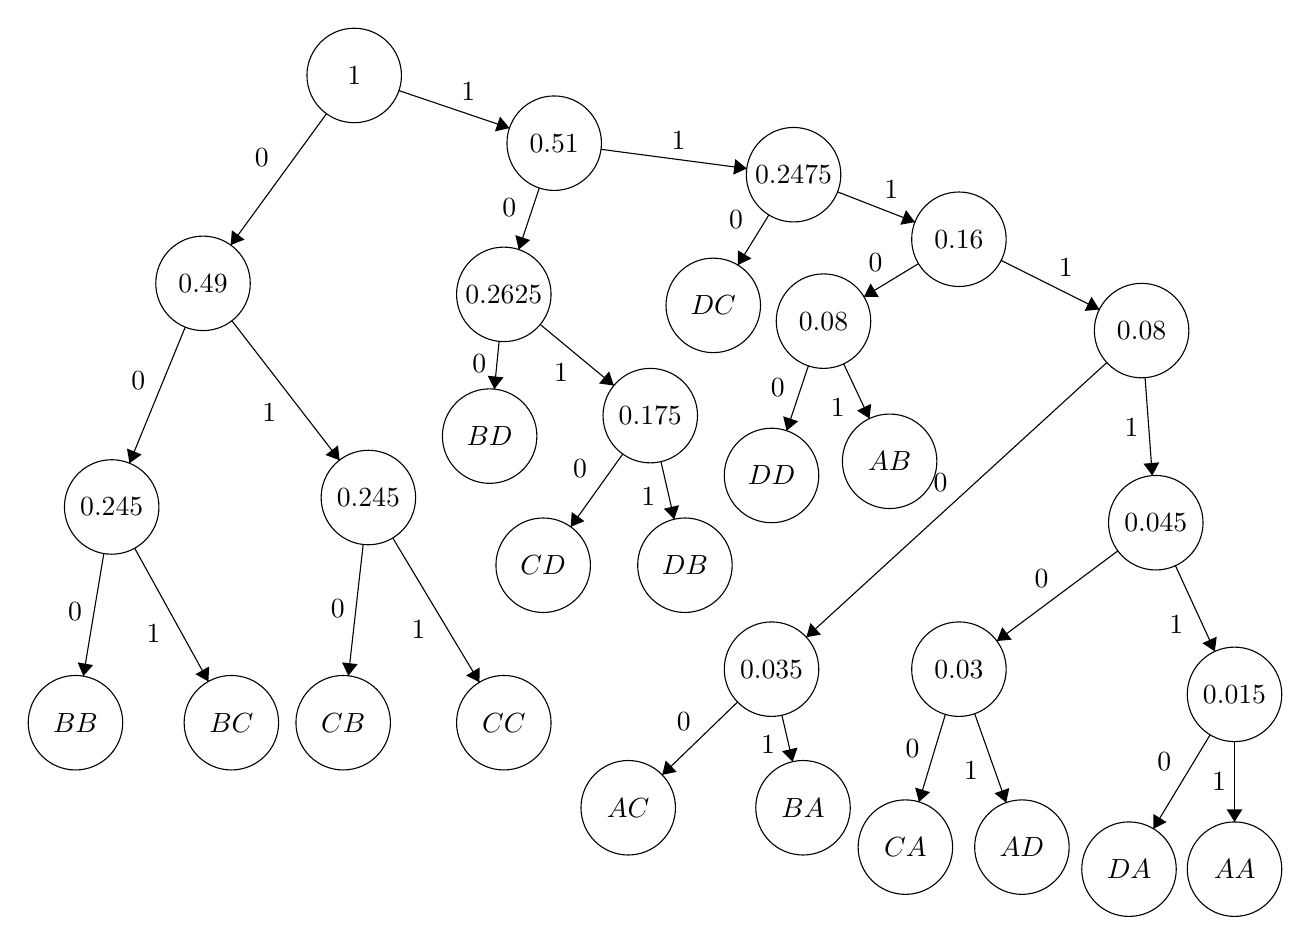
\begin{tikzpicture}[scale=0.2]
\tikzstyle{every node}+=[inner sep=0pt]
\draw [black] (20.9,-3.9) circle (3);
\draw (20.9,-3.9) node {$1$};
\draw [black] (11.3,-17.1) circle (3);
\draw (11.3,-17.1) node {$0.49$};
\draw [black] (5.5,-31.3) circle (3);
\draw (5.5,-31.3) node {$0.245$};
\draw [black] (21.8,-30.7) circle (3);
\draw (21.8,-30.7) node {$0.245$};
\draw [black] (3.2,-45) circle (3);
\draw (3.2,-45) node {$BB$};
\draw [black] (13.1,-45) circle (3);
\draw (13.1,-45) node {$BC$};
\draw [black] (20.2,-45) circle (3);
\draw (20.2,-45) node {$CB$};
\draw [black] (30.4,-45) circle (3);
\draw (30.4,-45) node {$CC$};
\draw [black] (33.6,-8.2) circle (3);
\draw (33.6,-8.2) node {$0.51$};
\draw [black] (30.4,-17.8) circle (3);
\draw (30.4,-17.8) node {$0.2625$};
\draw [black] (48.8,-10.2) circle (3);
\draw (48.8,-10.2) node {$0.2475$};
\draw [black] (29.5,-26.8) circle (3);
\draw (29.5,-26.8) node {$BD$};
\draw [black] (39.7,-25.5) circle (3);
\draw (39.7,-25.5) node {$0.175$};
\draw [black] (32.9,-35) circle (3);
\draw (32.9,-35) node {$CD$};
\draw [black] (41.9,-35) circle (3);
\draw (41.9,-35) node {$DB$};
\draw [black] (43.7,-18.5) circle (3);
\draw (43.7,-18.5) node {$DC$};
\draw [black] (59.3,-14.3) circle (3);
\draw (59.3,-14.3) node {$0.16$};
\draw [black] (50.7,-19.5) circle (3);
\draw (50.7,-19.5) node {$0.08$};
\draw [black] (70.9,-20.1) circle (3);
\draw (70.9,-20.1) node {$0.08$};
\draw [black] (47.4,-29.3) circle (3);
\draw (47.4,-29.3) node {$DD$};
\draw [black] (54.9,-28.4) circle (3);
\draw (54.9,-28.4) node {$AB$};
\draw [black] (47.4,-41.6) circle (3);
\draw (47.4,-41.6) node {$0.035$};
\draw [black] (71.8,-32.3) circle (3);
\draw (71.8,-32.3) node {$0.045$};
\draw [black] (38.3,-50.4) circle (3);
\draw (38.3,-50.4) node {$AC$};
\draw [black] (49.4,-50.4) circle (3);
\draw (49.4,-50.4) node {$BA$};
\draw [black] (59.3,-41.6) circle (3);
\draw (59.3,-41.6) node {$0.03$};
\draw [black] (76.8,-43.2) circle (3);
\draw (76.8,-43.2) node {$0.015$};
\draw [black] (55.9,-52.9) circle (3);
\draw (55.9,-52.9) node {$CA$};
\draw [black] (63.3,-52.9) circle (3);
\draw (63.3,-52.9) node {$AD$};
\draw [black] (70.1,-54.3) circle (3);
\draw (70.1,-54.3) node {$DA$};
\draw [black] (76.8,-54.3) circle (3);
\draw (76.8,-54.3) node {$AA$};
\draw [black] (19.14,-6.33) -- (13.06,-14.67);
\fill [black] (13.06,-14.67) -- (13.94,-14.32) -- (13.13,-13.73);
\draw (15.51,-9.12) node [left] {$0$};
\draw [black] (10.17,-19.88) -- (6.63,-28.52);
\fill [black] (6.63,-28.52) -- (7.4,-27.97) -- (6.47,-27.59);
\draw (7.66,-23.29) node [left] {$0$};
\draw [black] (13.13,-19.47) -- (19.97,-28.33);
\fill [black] (19.97,-28.33) -- (19.87,-27.39) -- (19.08,-28);
\draw (15.98,-25.31) node [left] {$1$};
\draw [black] (5,-34.26) -- (3.7,-42.04);
\fill [black] (3.7,-42.04) -- (4.32,-41.34) -- (3.34,-41.17);
\draw (3.64,-37.92) node [left] {$0$};
\draw [black] (6.96,-33.92) -- (11.64,-42.38);
\fill [black] (11.64,-42.38) -- (11.69,-41.43) -- (10.82,-41.92);
\draw (8.63,-39.35) node [left] {$1$};
\draw [black] (21.47,-33.68) -- (20.53,-42.02);
\fill [black] (20.53,-42.02) -- (21.12,-41.28) -- (20.13,-41.17);
\draw (20.34,-37.74) node [left] {$0$};
\draw [black] (23.35,-33.27) -- (28.85,-42.43);
\fill [black] (28.85,-42.43) -- (28.87,-41.49) -- (28.01,-42);
\draw (25.46,-39.11) node [left] {$1$};
\draw [black] (23.74,-4.86) -- (30.76,-7.24);
\fill [black] (30.76,-7.24) -- (30.16,-6.51) -- (29.84,-7.45);
\draw (28.15,-5.52) node [above] {$1$};
\draw [black] (32.65,-11.05) -- (31.35,-14.95);
\fill [black] (31.35,-14.95) -- (32.08,-14.35) -- (31.13,-14.04);
\draw (31.23,-12.3) node [left] {$0$};
\draw [black] (30.1,-20.79) -- (29.8,-23.81);
\fill [black] (29.8,-23.81) -- (30.38,-23.07) -- (29.38,-22.97);
\draw (29.31,-22.21) node [left] {$0$};
\draw [black] (32.71,-19.71) -- (37.39,-23.59);
\fill [black] (37.39,-23.59) -- (37.09,-22.69) -- (36.45,-23.46);
\draw (34.04,-22.14) node [below] {$1$};
\draw [black] (37.95,-27.94) -- (34.65,-32.56);
\fill [black] (34.65,-32.56) -- (35.52,-32.2) -- (34.71,-31.62);
\draw (35.71,-28.88) node [left] {$0$};
\draw [black] (40.38,-28.42) -- (41.22,-32.08);
\fill [black] (41.22,-32.08) -- (41.53,-31.19) -- (40.56,-31.41);
\draw (40.05,-30.65) node [left] {$1$};
\draw [black] (36.57,-8.59) -- (45.83,-9.81);
\fill [black] (45.83,-9.81) -- (45.1,-9.21) -- (44.97,-10.2);
\draw (41.5,-8.61) node [above] {$1$};
\draw [black] (47.23,-12.76) -- (45.27,-15.94);
\fill [black] (45.27,-15.94) -- (46.12,-15.52) -- (45.26,-15);
\draw (45.62,-13.07) node [left] {$0$};
\draw [black] (51.59,-11.29) -- (56.51,-13.21);
\fill [black] (56.51,-13.21) -- (55.94,-12.45) -- (55.58,-13.38);
\draw (55,-11.73) node [above] {$1$};
\draw [black] (56.73,-15.85) -- (53.27,-17.95);
\fill [black] (53.27,-17.95) -- (54.21,-17.96) -- (53.69,-17.11);
\draw (54,-16.4) node [above] {$0$};
\draw [black] (61.98,-15.64) -- (68.22,-18.76);
\fill [black] (68.22,-18.76) -- (67.72,-17.95) -- (67.28,-18.85);
\draw (66.09,-16.7) node [above] {$1$};
\draw [black] (49.74,-22.34) -- (48.36,-26.46);
\fill [black] (48.36,-26.46) -- (49.09,-25.86) -- (48.14,-25.54);
\draw (48.28,-23.69) node [left] {$0$};
\draw [black] (51.98,-22.21) -- (53.62,-25.69);
\fill [black] (53.62,-25.69) -- (53.73,-24.75) -- (52.83,-25.18);
\draw (52.09,-25) node [left] {$1$};
\draw [black] (68.69,-22.13) -- (49.61,-39.57);
\fill [black] (49.61,-39.57) -- (50.54,-39.4) -- (49.87,-38.67);
\draw (58.14,-30.36) node [above] {$0$};
\draw [black] (71.12,-23.09) -- (71.58,-29.31);
\fill [black] (71.58,-29.31) -- (72.02,-28.47) -- (71.02,-28.55);
\draw (70.74,-26.25) node [left] {$1$};
\draw [black] (45.24,-43.69) -- (40.46,-48.31);
\fill [black] (40.46,-48.31) -- (41.38,-48.12) -- (40.68,-47.4);
\draw (41.83,-45.52) node [above] {$0$};
\draw [black] (48.06,-44.53) -- (48.74,-47.47);
\fill [black] (48.74,-47.47) -- (49.05,-46.58) -- (48.07,-46.81);
\draw (47.65,-46.39) node [left] {$1$};
\draw [black] (69.39,-34.09) -- (61.71,-39.81);
\fill [black] (61.71,-39.81) -- (62.65,-39.73) -- (62.05,-38.93);
\draw (64.55,-36.45) node [above] {$0$};
\draw [black] (73.05,-35.03) -- (75.55,-40.47);
\fill [black] (75.55,-40.47) -- (75.67,-39.54) -- (74.76,-39.95);
\draw (73.58,-38.77) node [left] {$1$};
\draw [black] (58.44,-44.47) -- (56.76,-50.03);
\fill [black] (56.76,-50.03) -- (57.47,-49.41) -- (56.52,-49.12);
\draw (56.83,-46.64) node [left] {$0$};
\draw [black] (60.3,-44.43) -- (62.3,-50.07);
\fill [black] (62.3,-50.07) -- (62.5,-49.15) -- (61.56,-49.48);
\draw (60.54,-48.01) node [left] {$1$};
\draw [black] (75.25,-45.77) -- (71.65,-51.73);
\fill [black] (71.65,-51.73) -- (72.49,-51.31) -- (71.64,-50.79);
\draw (72.81,-47.48) node [left] {$0$};
\draw [black] (76.8,-46.2) -- (76.8,-51.3);
\fill [black] (76.8,-51.3) -- (77.3,-50.5) -- (76.3,-50.5);
\draw (76.3,-48.75) node [left] {$1$};
\end{tikzpicture}
\end{center}

Kodiranja su sljedeća:

BB - 000, BC - 001, CB - 010, CC - 011, BD - 100, DC - 110

CD - 1010, DB - 1011, DD - 11100, AB - 11101, AC - 111100, BA - 111101

CA - 1111100, AD - 1111101, DA - 1111110, AA - 1111111

$$H(X/X^{\infty}) = - \frac{1}{\ln{2}} \sum_{i = 1}^{16} p_i \ln{p_i} \approx 3.5526$$
$$n_{sr} = \sum_{i = 1}^{16} p_i n_i = 3.62$$

Protok:

$$\overline{I(X)} = \frac{0.9814}{\tau}$$

Tj. $98.14\%$

Poruka: ADBBAAADDC

$$111110100011111111111101110$$

\newpage

d)\\

$m = 2, m^{*} = 2$

Zadatak je urađen u 14 iteracija, ovdje ćemo prikazati njih 5(ostale ćemo preskočiti):

\begin{table}[hp]
\hspace*{-1.25in}
\begin{tabular}{|l|l|l|l|l|l|l|l|l|l|l|l|}
\hline
\multicolumn{2}{|l|}{Početak} & \multicolumn{2}{l|}{Iteracija 1} & \multicolumn{2}{l|}{Iteracija 2} & \multicolumn{2}{l|}{Iteracija 3} & \multicolumn{2}{l|}{Iteracija 4} & \multicolumn{2}{l|}{Iteracija 5} \\ \hline
BB & 0.1225 & BB & 0.1225 & CD/0 & \multirow{2}{*}{0.175} & CB/0 & \multirow{2}{*}{0.245} & BB/00 & \multirow{10}{*}{0.43} & CD/0000 & \multirow{16}{*}{1} \\ \cline{1-5}
BC & 0.1225 & BC & 0.1225 & DB/1 &  & CC/1 &  & BC/01 &  & DB/0001 &  \\ \cline{1-8}
CB & 0.1225 & CB & 0.1225 & DC/0 & \multirow{2}{*}{0.15} & BB/0 & \multirow{2}{*}{0.245} & AB/10000 &  & DC/0010 &  \\ \cline{1-5}
CC & 0.1225 & CC & 0.1225 & DD/1 &  & BC/1 &  & AC/10001 &  & DD/0011 &  \\ \cline{1-8}
BD & 0.0875 & BD & 0.0875 & BB & 0.1225 & AB/0000 & \multirow{8}{*}{0.185} & DA/100100 &  & CB/010 &  \\ \cline{1-6}
CD & 0.0875 & CD & 0.0875 & BC & 0.1225 & AC/0001 &  & AA/100101 &  & CC/011 &  \\ \cline{1-6}
DB & 0.0875 & DB & 0.0875 & CB & 0.1225 & DA/00100 &  & AD/10011 &  & BB/100 &  \\ \cline{1-6}
DC & 0.0875 & DC & 0.0875 & CC & 0.1225 & AA/00101 &  & BA/1010 &  & BC/101 &  \\ \cline{1-6}
DD & 0.0625 & DD & 0.0625 & AB/000 & \multirow{7}{*}{0.0975} & AD/0011 &  & CA/1011 &  & AB/110000 &  \\ \cline{1-4}
AB & 0.0175 & BA/0 & \multirow{2}{*}{0.035} & AC/001 &  & BA/010 &  & BD/11 &  & AC/110001 &  \\ \cline{1-2} \cline{9-10}
AC & 0.0175 & CA/1 &  & DA/0100 &  & CA/011 &  & CD/00 & \multirow{4}{*}{0.325} & DA/1100100 &  \\ \cline{1-4}
BA & 0.0175 & AB/0 & \multirow{2}{*}{0.035} & AA/0101 &  & BD/1 &  & DB/01 &  & AA/1100101 &  \\ \cline{1-2} \cline{7-8}
CA & 0.0175 & AC/1 &  & AD/011 &  & CD/0 & \multirow{2}{*}{0.175} & DC/10 &  & AD/110011 &  \\ \cline{1-4}
AD & 0.0125 & DA/00 & \multirow{3}{*}{0.0275} & BA/10 &  & DB/1 &  & DD/11 &  & BA/11010 &  \\ \cline{1-2} \cline{7-10}
DA & 0.0125 & AA/01 &  & CA/11 &  & DC/0 & \multirow{2}{*}{0.15} & CB/0 & \multirow{2}{*}{0.245} & CA/11011 &  \\ \cline{1-2} \cline{5-6} \cline{9-9}
AA & 0.0025 & AD/1 &  & BD & 0.0875 & DD/1 &  & CC/1 &  & BD/111 &  \\ \hline
\end{tabular}
\end{table}

$$H(X/X^{\infty}) = - \frac{1}{\ln{2}} \sum_{i = 1}^{16} p_i \ln{p_i} \approx 3.5526$$
$$n_{sr} = 3.5975$$

$$\overline{I(X)} = \frac{0.9875}{\tau}$$

Iskoristivost kanala veze 98.75\%

Poruka: ADBBAAADDC

$$11001110011001011100110010$$

\newpage

\section*{Zadatak 7\label{Z7}}

\underline{Postavka:}

Markovljev izvor informacija prvog reda emitira tri različite poruke a, b i c. Ovisno od toga koja je poruka posljednja emitirana, izvor se nalazi u jednom od 3 moguća stanja Sa, Sb i Sc koja redom odgovaraju emitiranim porukama a, b odnosno c. Vjerovatnoće da će izvor emitirati neku od ove 3 poruke ovisno od stanja u kojem se nalazi date su u sljedećoj tablici: 

\begin{table}[hp]
\centering
\begin{tabular}{|l|l|l|l|}
\hline
p($x_j$ / $S_i$) & a & b & c \\ \hline
$S_a$ & 0.3 & 0.3 & 0.4 \\ \hline
$S_b$ & 0.2 & 0.3 & 0.5 \\ \hline
$S_c$ & 0.1 & 0.1 & 0.8 \\ \hline
\end{tabular}
\end{table}

Za ovaj izvor informacija formirajte binarni Shannon-Fano kod sa simbolima 0 i 1

a) posmatrajući izvor kao izvor bez memorije;

b) posmatrajući izvor kao izvor bez memorije, ali kodirajući parove poruka umjesto individualnih poruka;

c) koristeći posebno kodiranje za svako stanje;

d) koristeći posebno kodiranje za svako stanje, ali kodirajući parove poruka umjesto individualnih poruka.

Za sva četiri načina kodiranja, izračunajte protok informacija kroz komunikacioni kanal, procenat iskorištenja kanala veze, te kodirajte sekvencu poruka baacbcbbbbaaab. U posljednja dva slučaja, pretpostavite da izvor započinje rad u stanju Sa.

\underline{Rješenje:}\\

\begin{center}
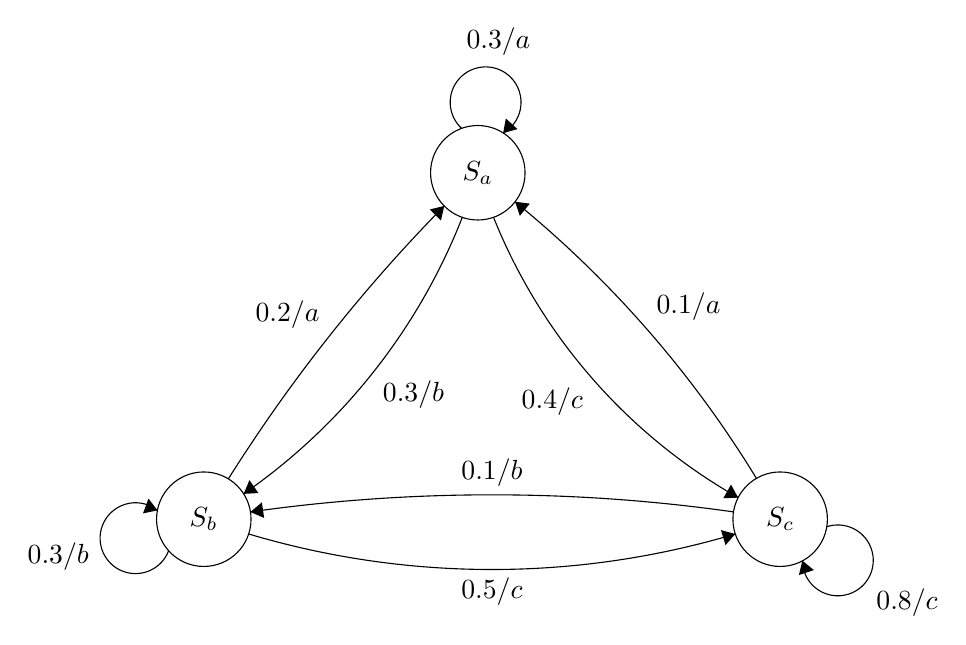
\begin{tikzpicture}[scale=0.2]
\tikzstyle{every node}+=[inner sep=0pt]
\draw [black] (34.2,-14.4) circle (3);
\draw (34.2,-14.4) node {$S_a$};
\draw [black] (16.8,-36.4) circle (3);
\draw (16.8,-36.4) node {$S_b$};
\draw [black] (53.4,-36.4) circle (3);
\draw (53.4,-36.4) node {$S_c$};
\draw [black] (33.215,-17.233) arc (-21.40272:-55.27887:38.415);
\fill [black] (19.33,-34.79) -- (20.27,-34.74) -- (19.7,-33.92);
\draw (28.14,-28.46) node [right] {$0.3/b$};
\draw [black] (18.36,-33.838) arc (147.82641:135.492:102.83);
\fill [black] (32.07,-16.51) -- (31.15,-16.73) -- (31.86,-17.43);
\draw (24.18,-23.39) node [left] {$0.2/a$};
\draw [black] (14.572,-38.391) arc (-20.47589:-308.47589:2.25);
\draw (9.53,-38.75) node [left] {$0.3/b$};
\fill [black] (13.86,-35.84) -- (13.29,-35.09) -- (12.94,-36.03);
\draw [black] (50.551,-37.338) arc (-73.37642:-106.62358:54.008);
\fill [black] (50.55,-37.34) -- (49.64,-37.09) -- (49.93,-38.05);
\draw (35.1,-40.09) node [below] {$0.5/c$};
\draw [black] (50.733,-35.029) arc (-119.61245:-158.16337:35.785);
\fill [black] (50.73,-35.03) -- (50.28,-34.2) -- (49.79,-35.07);
\draw (40.91,-28.9) node [left] {$0.4/c$};
\draw [black] (36.566,-16.244) arc (50.83296:31.39122:69.026);
\fill [black] (36.57,-16.24) -- (36.87,-17.14) -- (37.5,-16.36);
\draw (45.52,-22.92) node [right] {$0.1/a$};
\draw [black] (56.349,-36.881) arc (108.46232:-179.53768:2.25);
\draw (59.48,-41.7) node [right] {$0.8/c$};
\fill [black] (54.81,-39.03) -- (54.59,-39.95) -- (55.54,-39.63);
\draw [black] (33.181,-11.591) arc (227.65981:-60.34019:2.25);
\draw (35.51,-6.98) node [above] {$0.3/a$};
\fill [black] (35.81,-11.88) -- (36.72,-11.63) -- (35.98,-10.95);
\draw [black] (19.764,-35.936) arc (98.10324:81.89676:108.8);
\fill [black] (19.76,-35.94) -- (20.63,-36.32) -- (20.49,-35.33);
\draw (35.1,-34.35) node [above] {$0.1/b$};
\end{tikzpicture}
\end{center}

Potrebno je riješiti sljedeći sistem jednačina:

$$-0.7 p(S_a) + 0.2p(S_b) + 0.1p(S_c) = 0$$
$$0.3p(S_a) - 0.7p(S_b) + 0.1p(S_c) = 0$$
$$p(S_a) + p(S_b) + p(S_c) = 1$$

Rješavamo svođenjem matrice na desnu trougaonu matricu, te dobijemo:

$$p(S_a) = 0.145$$
$$p(S_b) = 0.161$$
$$p(S_c) = 0.693$$

Pa je:

$$H(S_a) = - \frac{1}{\ln{2}} (p(a/S_a) \ln{p(a/S_a)} + p(b/S_a) \ln{p(b/S_a)} + p(c/S_a) \ln{p(c/S_a)}) = 1.57095$$
$$H(S_b) = 1.48548$$
$$H(S_c) = 0.921928$$

$$H(X/X^{\infty}) = \sum_{i = 1}^{3} p(S_i)H(S_i) = 1.10585$$

Prelazimo na rješavanje ostatka zadatka:

\newpage
a)\\

\begin{table}[hp]
\centering
\begin{tabular}{|l|l|l|l}
\cline{1-3}
c & 0.693 & 0.693/0 &  \\ \hline
b & 0.161 & \multirow{2}{*}{0.306/1} & \multicolumn{1}{l|}{0.161/10} \\ \cline{1-2} \cline{4-4} 
a & 0.145 &  & \multicolumn{1}{l|}{0.145/11} \\ \hline
\end{tabular}
\end{table}

$$n_{sr} = 1.305$$
$$\overline{I(X)} = \frac{0.8474}{\tau}$$

Iskorištenost kanala veze 84.74\%

Poruka: baacbcbbbbaaab

$$10111101001010101011111110$$

\newpage
b)\\

Sortirane vjerovatnoće pojavljivanja parova poruka:

\begin{table}[hp]
\centering
\begin{tabular}{|l|l|}
\hline
cc & 0.480 \\ \hline
bc & 0.1115 \\ \hline
cb & 0.1115 \\ \hline
ca & 0.1004 \\ \hline
ac & 0.1004 \\ \hline
bb & 0.02592 \\ \hline
ab & 0.0233 \\ \hline
ba & 0.0233 \\ \hline
aa & 0.0210 \\ \hline
\end{tabular}
\end{table}

Kodiramo pomoću binarnog stabla:

\begin{center}
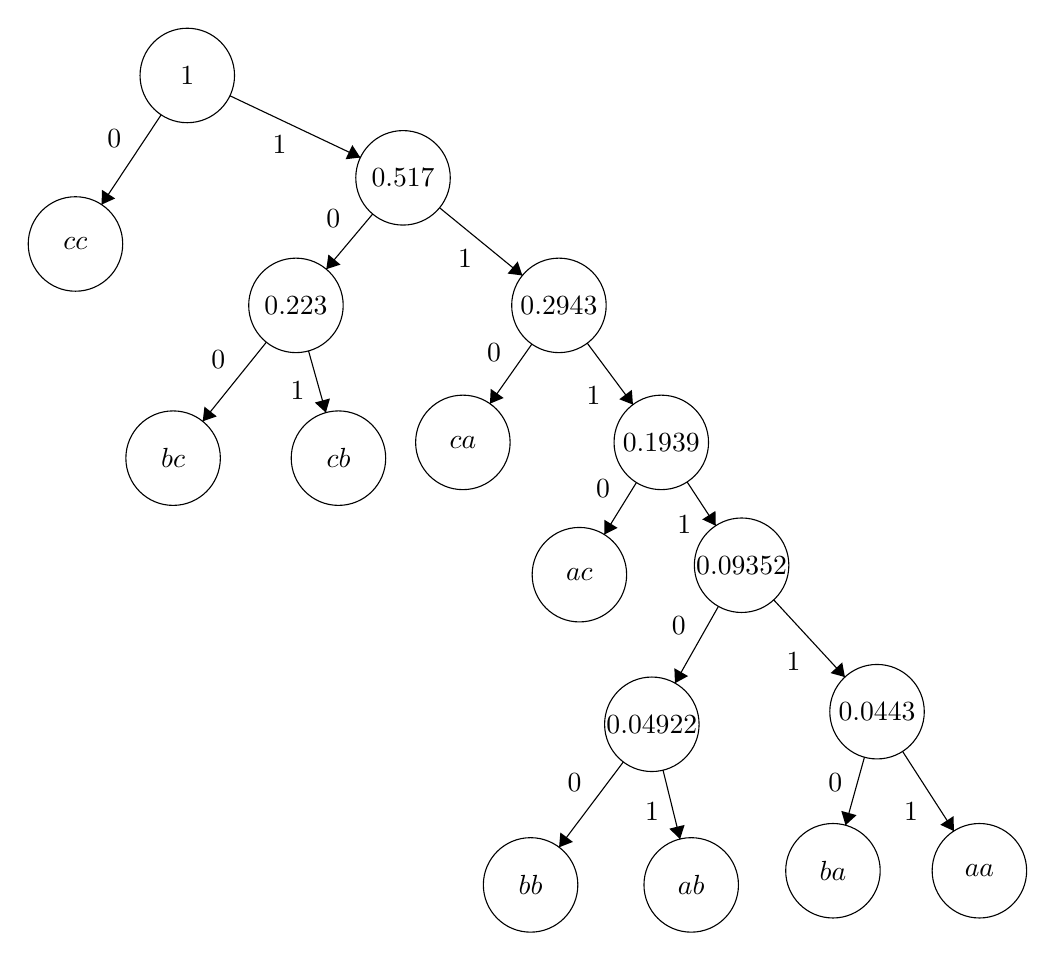
\begin{tikzpicture}[scale=0.2]
\tikzstyle{every node}+=[inner sep=0pt]
\draw [black] (20.9,-4.6) circle (3);
\draw (20.9,-4.6) node {$1$};
\draw [black] (13.8,-15.3) circle (3);
\draw (13.8,-15.3) node {$cc$};
\draw [black] (34.6,-11.1) circle (3);
\draw (34.6,-11.1) node {$0.517$};
\draw [black] (27.8,-19.2) circle (3);
\draw (27.8,-19.2) node {$0.223$};
\draw [black] (44.5,-19.2) circle (3);
\draw (44.5,-19.2) node {$0.2943$};
\draw [black] (51,-27.9) circle (3);
\draw (51,-27.9) node {$0.1939$};
\draw [black] (20,-28.9) circle (3);
\draw (20,-28.9) node {$bc$};
\draw [black] (30.5,-28.9) circle (3);
\draw (30.5,-28.9) node {$cb$};
\draw [black] (38.4,-27.9) circle (3);
\draw (38.4,-27.9) node {$ca$};
\draw [black] (45.8,-36.3) circle (3);
\draw (45.8,-36.3) node {$ac$};
\draw [black] (56.1,-35.7) circle (3);
\draw (56.1,-35.7) node {$0.09352$};
\draw [black] (50.4,-45.8) circle (3);
\draw (50.4,-45.8) node {$0.04922$};
\draw [black] (64.7,-45) circle (3);
\draw (64.7,-45) node {$0.0443$};
\draw [black] (42.7,-56) circle (3);
\draw (42.7,-56) node {$bb$};
\draw [black] (52.9,-56) circle (3);
\draw (52.9,-56) node {$ab$};
\draw [black] (61.9,-55.1) circle (3);
\draw (61.9,-55.1) node {$ba$};
\draw [black] (71.2,-55.1) circle (3);
\draw (71.2,-55.1) node {$aa$};
\draw [black] (19.24,-7.1) -- (15.46,-12.8);
\fill [black] (15.46,-12.8) -- (16.32,-12.41) -- (15.48,-11.86);
\draw (16.74,-8.62) node [left] {$0$};
\draw [black] (23.61,-5.89) -- (31.89,-9.81);
\fill [black] (31.89,-9.81) -- (31.38,-9.02) -- (30.95,-9.92);
\draw (26.76,-8.36) node [below] {$1$};
\draw [black] (32.67,-13.4) -- (29.73,-16.9);
\fill [black] (29.73,-16.9) -- (30.63,-16.61) -- (29.86,-15.97);
\draw (30.65,-13.71) node [left] {$0$};
\draw [black] (36.92,-13) -- (42.18,-17.3);
\fill [black] (42.18,-17.3) -- (41.88,-16.41) -- (41.24,-17.18);
\draw (38.54,-15.64) node [below] {$1$};
\draw [black] (25.92,-21.54) -- (21.88,-26.56);
\fill [black] (21.88,-26.56) -- (22.77,-26.25) -- (21.99,-25.63);
\draw (23.34,-22.63) node [left] {$0$};
\draw [black] (28.6,-22.09) -- (29.7,-26.01);
\fill [black] (29.7,-26.01) -- (29.96,-25.11) -- (29,-25.37);
\draw (28.38,-24.59) node [left] {$1$};
\draw [black] (42.78,-21.66) -- (40.12,-25.44);
\fill [black] (40.12,-25.44) -- (40.99,-25.08) -- (40.17,-24.5);
\draw (40.85,-22.19) node [left] {$0$};
\draw [black] (46.3,-21.6) -- (49.2,-25.5);
\fill [black] (49.2,-25.5) -- (49.13,-24.56) -- (48.33,-25.16);
\draw (47.17,-24.95) node [left] {$1$};
\draw [black] (49.42,-30.45) -- (47.38,-33.75);
\fill [black] (47.38,-33.75) -- (48.23,-33.33) -- (47.38,-32.81);
\draw (47.77,-30.81) node [left] {$0$};
\draw [black] (52.64,-30.41) -- (54.46,-33.19);
\fill [black] (54.46,-33.19) -- (54.44,-32.25) -- (53.6,-32.79);
\draw (52.93,-33.12) node [left] {$1$};
\draw [black] (54.63,-38.31) -- (51.87,-43.19);
\fill [black] (51.87,-43.19) -- (52.7,-42.74) -- (51.83,-42.24);
\draw (52.59,-39.54) node [left] {$0$};
\draw [black] (58.14,-37.9) -- (62.66,-42.8);
\fill [black] (62.66,-42.8) -- (62.49,-41.87) -- (61.75,-42.55);
\draw (59.87,-41.81) node [left] {$1$};
\draw [black] (48.59,-48.19) -- (44.51,-53.61);
\fill [black] (44.51,-53.61) -- (45.39,-53.27) -- (44.59,-52.67);
\draw (45.97,-49.5) node [left] {$0$};
\draw [black] (51.11,-48.71) -- (52.19,-53.09);
\fill [black] (52.19,-53.09) -- (52.48,-52.19) -- (51.51,-52.43);
\draw (50.89,-51.34) node [left] {$1$};
\draw [black] (63.9,-47.89) -- (62.7,-52.21);
\fill [black] (62.7,-52.21) -- (63.4,-51.57) -- (62.43,-51.3);
\draw (62.53,-49.51) node [left] {$0$};
\draw [black] (66.32,-47.52) -- (69.58,-52.58);
\fill [black] (69.58,-52.58) -- (69.56,-51.63) -- (68.72,-52.18);
\draw (67.33,-51.36) node [left] {$1$};
\end{tikzpicture}
\end{center}

Rezultat kodiranja:

cc - 0, bc - 100, cb - 101, ca - 110, ac - 1110, bb - 111100, ab - 111101, ba - 111110, aa - 111111

$$n_{sr} = 2.41292$$
$$\overline{I(X)} = \frac{0.9166}{\tau}$$

Iskorištenost kanala veze: 91.66\%

Poruka: baacbcbbbbaaab

$$1111101110100111100111100111111111101$$

\newpage
c)\\

Za $S_a$

\begin{table}[hp]
\centering
\begin{tabular}{|l|l|l|l}
\cline{1-3}
c & 0.4 & 0.4/0 &  \\ \hline
b & 0.3 & \multirow{2}{*}{0.6/1} & \multicolumn{1}{l|}{0.3/10} \\ \cline{1-2} \cline{4-4} 
a & 0.3 &  & \multicolumn{1}{l|}{0.3/11} \\ \hline
\end{tabular}
\end{table}

c - 0, b - 10, a - 11

$$n_{sr} = 1.6$$


Za $S_b$

\begin{table}[hp]
\centering
\begin{tabular}{|l|l|l|l}
\cline{1-3}
c & 0.5 & 0.5/0 &  \\ \hline
b & 0.3 & \multirow{2}{*}{0.5/1} & \multicolumn{1}{l|}{0.3/10} \\ \cline{1-2} \cline{4-4} 
a & 0.2 &  & \multicolumn{1}{l|}{0.2/11} \\ \hline
\end{tabular}
\end{table}

c - 0, b - 10, a - 11

$$n_{sr} = 1.5$$


Za $S_c$

\begin{table}[hp]
\centering
\begin{tabular}{|l|l|l|l}
\cline{1-3}
c & 0.8 & 0.8/0 &  \\ \hline
b & 0.1 & \multirow{2}{*}{0.2/1} & \multicolumn{1}{l|}{0.1/10} \\ \cline{1-2} \cline{4-4} 
a & 0.1 &  & \multicolumn{1}{l|}{0.1/11} \\ \hline
\end{tabular}
\end{table}

c - 0, b - 10, a - 11

$$n_{sr} = 1.2$$

Po svim stanjima: $$n_{sr} = 0.145 \cdot 1.6 + 0.161 \cdot 1.5 + 0.693 \cdot 1.2 = 1.3051$$

$$\overline{I(X)} = \frac{0.8473}{\tau}$$
Iskorištenost: 84.73\%

Poruka za $S_a = S_b = S_c$  jer im je isto kodiranje:

$$10111101001010101011111110$$

\newpage
d)\\

Za sva stanja kodiramo pomoću stabla:

Za $S_a$

\begin{center}
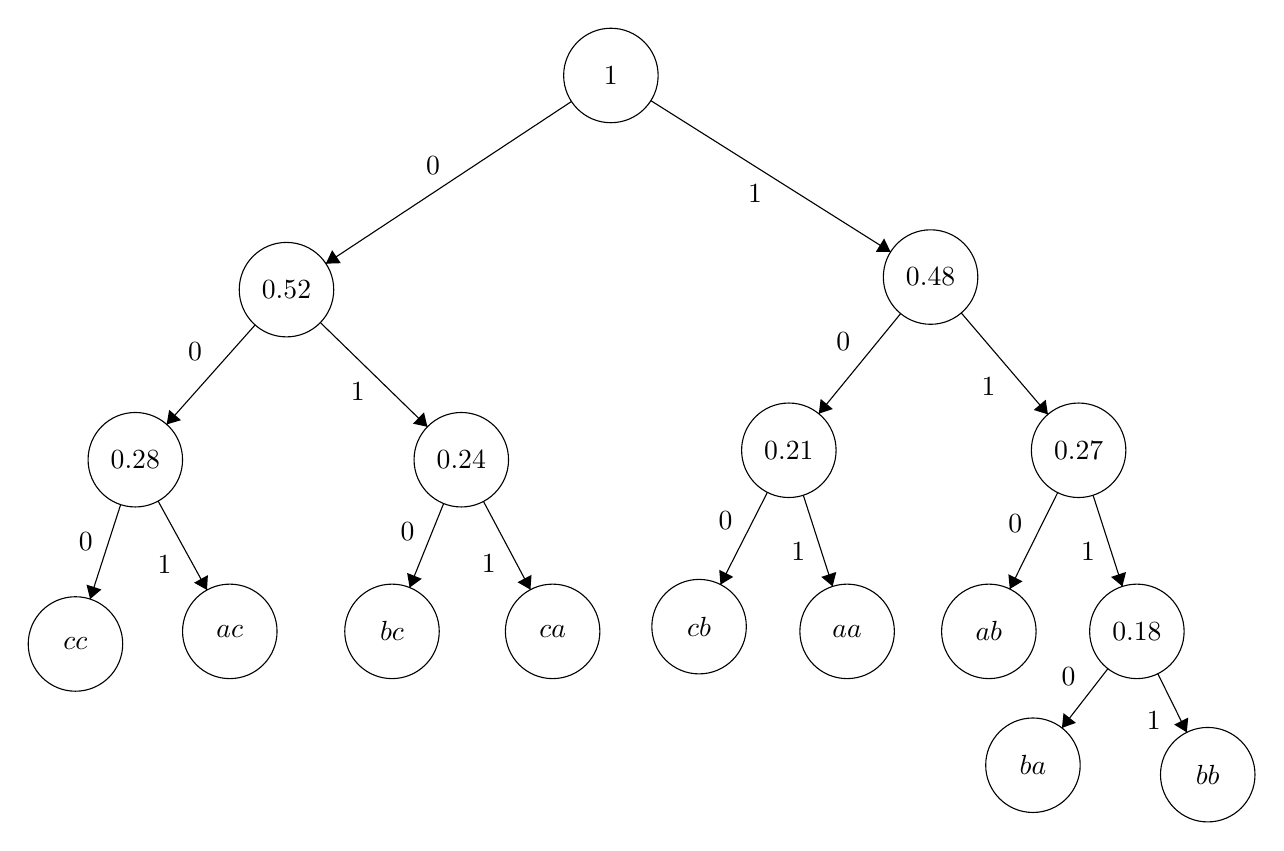
\begin{tikzpicture}[scale=0.2]
\tikzstyle{every node}+=[inner sep=0pt]
\draw [black] (38.7,-5.8) circle (3);
\draw (38.7,-5.8) node {$1$};
\draw [black] (18.1,-19.4) circle (3);
\draw (18.1,-19.4) node {$0.52$};
\draw [black] (59,-18.6) circle (3);
\draw (59,-18.6) node {$0.48$};
\draw [black] (8.5,-30.2) circle (3);
\draw (8.5,-30.2) node {$0.28$};
\draw [black] (29.2,-30.2) circle (3);
\draw (29.2,-30.2) node {$0.24$};
\draw [black] (50,-29.6) circle (3);
\draw (50,-29.6) node {$0.21$};
\draw [black] (68.4,-29.6) circle (3);
\draw (68.4,-29.6) node {$0.27$};
\draw [black] (4.7,-41.9) circle (3);
\draw (4.7,-41.9) node {$cc$};
\draw [black] (14.5,-41.1) circle (3);
\draw (14.5,-41.1) node {$ac$};
\draw [black] (24.8,-41.1) circle (3);
\draw (24.8,-41.1) node {$bc$};
\draw [black] (35,-41.1) circle (3);
\draw (35,-41.1) node {$ca$};
\draw [black] (44.3,-40.8) circle (3);
\draw (44.3,-40.8) node {$cb$};
\draw [black] (53.7,-41.1) circle (3);
\draw (53.7,-41.1) node {$aa$};
\draw [black] (62.7,-41.1) circle (3);
\draw (62.7,-41.1) node {$ab$};
\draw [black] (72.1,-41.1) circle (3);
\draw (72.1,-41.1) node {$0.18$};
\draw [black] (65.5,-49.6) circle (3);
\draw (65.5,-49.6) node {$ba$};
\draw [black] (76.6,-50.2) circle (3);
\draw (76.6,-50.2) node {$bb$};
\draw [black] (36.2,-7.45) -- (20.6,-17.75);
\fill [black] (20.6,-17.75) -- (21.55,-17.72) -- (21,-16.89);
\draw (27.4,-12.1) node [above] {$0$};
\draw [black] (41.24,-7.4) -- (56.46,-17);
\fill [black] (56.46,-17) -- (56.05,-16.15) -- (55.52,-17);
\draw (47.85,-12.7) node [below] {$1$};
\draw [black] (16.11,-21.64) -- (10.49,-27.96);
\fill [black] (10.49,-27.96) -- (11.4,-27.69) -- (10.65,-27.03);
\draw (12.76,-23.35) node [left] {$0$};
\draw [black] (20.25,-21.49) -- (27.05,-28.11);
\fill [black] (27.05,-28.11) -- (26.83,-27.19) -- (26.13,-27.91);
\draw (22.63,-25.28) node [below] {$1$};
\draw [black] (57.1,-20.92) -- (51.9,-27.28);
\fill [black] (51.9,-27.28) -- (52.79,-26.98) -- (52.02,-26.34);
\draw (53.94,-22.67) node [left] {$0$};
\draw [black] (60.95,-20.88) -- (66.45,-27.32);
\fill [black] (66.45,-27.32) -- (66.31,-26.39) -- (65.55,-27.04);
\draw (63.15,-25.54) node [left] {$1$};
\draw [black] (7.57,-33.05) -- (5.63,-39.05);
\fill [black] (5.63,-39.05) -- (6.35,-38.44) -- (5.4,-38.13);
\draw (5.83,-35.37) node [left] {$0$};
\draw [black] (9.95,-32.83) -- (13.05,-38.47);
\fill [black] (13.05,-38.47) -- (13.11,-37.53) -- (12.23,-38.01);
\draw (10.83,-36.84) node [left] {$1$};
\draw [black] (28.08,-32.98) -- (25.92,-38.32);
\fill [black] (25.92,-38.32) -- (26.69,-37.76) -- (25.76,-37.39);
\draw (26.26,-34.76) node [left] {$0$};
\draw [black] (30.61,-32.85) -- (33.59,-38.45);
\fill [black] (33.59,-38.45) -- (33.66,-37.51) -- (32.77,-37.98);
\draw (31.42,-36.81) node [left] {$1$};
\draw [black] (48.64,-32.27) -- (45.66,-38.13);
\fill [black] (45.66,-38.13) -- (46.47,-37.64) -- (45.58,-37.19);
\draw (46.46,-34.08) node [left] {$0$};
\draw [black] (50.92,-32.46) -- (52.78,-38.24);
\fill [black] (52.78,-38.24) -- (53.01,-37.33) -- (52.06,-37.64);
\draw (51.08,-36.02) node [left] {$1$};
\draw [black] (67.07,-32.29) -- (64.03,-38.41);
\fill [black] (64.03,-38.41) -- (64.84,-37.92) -- (63.94,-37.47);
\draw (64.85,-34.25) node [left] {$0$};
\draw [black] (69.32,-32.46) -- (71.18,-38.24);
\fill [black] (71.18,-38.24) -- (71.41,-37.33) -- (70.46,-37.64);
\draw (69.48,-36.02) node [left] {$1$};
\draw [black] (70.26,-43.47) -- (67.34,-47.23);
\fill [black] (67.34,-47.23) -- (68.23,-46.91) -- (67.44,-46.29);
\draw (68.23,-43.94) node [left] {$0$};
\draw [black] (73.43,-43.79) -- (75.27,-47.51);
\fill [black] (75.27,-47.51) -- (75.36,-46.57) -- (74.47,-47.02);
\draw (73.65,-46.75) node [left] {$1$};
\end{tikzpicture}
\end{center}

$$n_{sr} = 3.18$$

Poruka: baacbcbbbbaaab

$$111000101011111111101110$$

Za $S_b$

\begin{center}
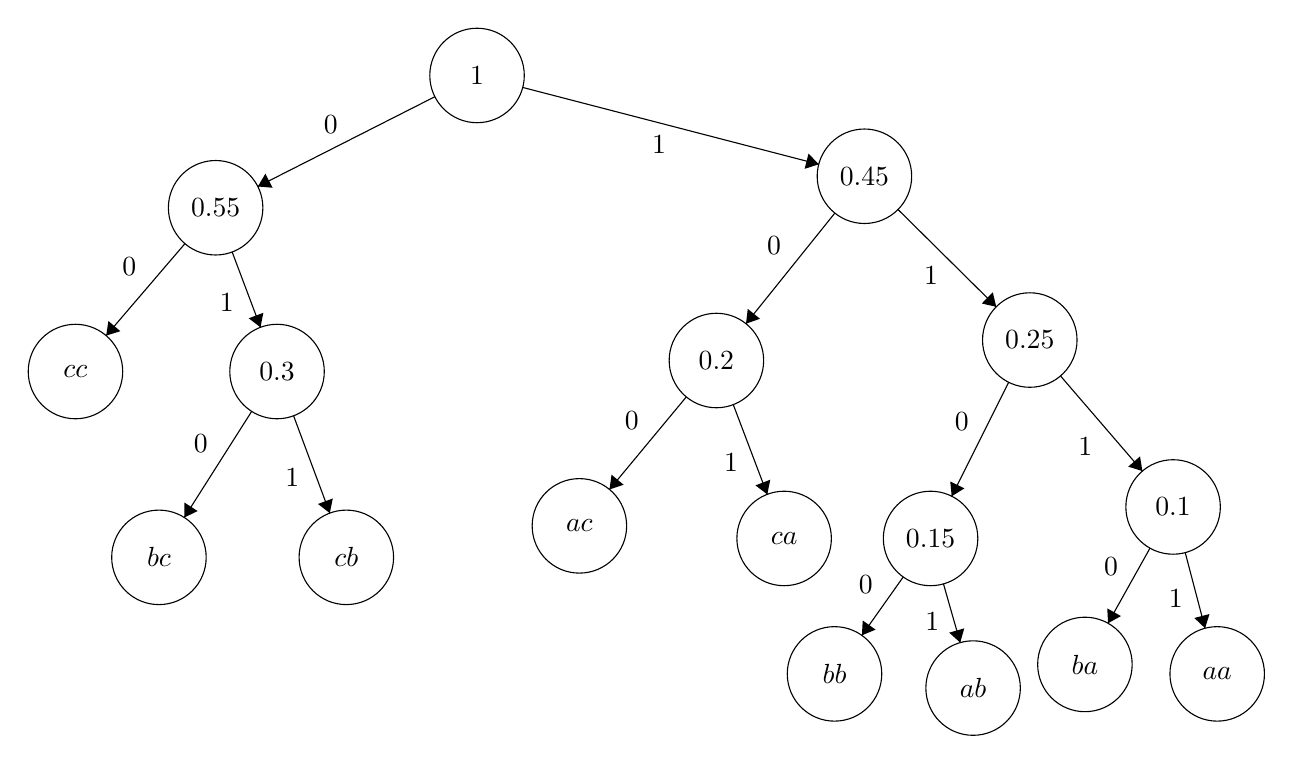
\begin{tikzpicture}[scale=0.2]
\tikzstyle{every node}+=[inner sep=0pt]
\draw [black] (30.1,-4.9) circle (3);
\draw (30.1,-4.9) node {$1$};
\draw [black] (13.5,-13.3) circle (3);
\draw (13.5,-13.3) node {$0.55$};
\draw [black] (54.7,-11.3) circle (3);
\draw (54.7,-11.3) node {$0.45$};
\draw [black] (4.6,-23.7) circle (3);
\draw (4.6,-23.7) node {$cc$};
\draw [black] (17.4,-23.7) circle (3);
\draw (17.4,-23.7) node {$0.3$};
\draw [black] (9.9,-35.5) circle (3);
\draw (9.9,-35.5) node {$bc$};
\draw [black] (21.8,-35.5) circle (3);
\draw (21.8,-35.5) node {$cb$};
\draw [black] (45.3,-23) circle (3);
\draw (45.3,-23) node {$0.2$};
\draw [black] (65.2,-21.7) circle (3);
\draw (65.2,-21.7) node {$0.25$};
\draw [black] (36.6,-33.5) circle (3);
\draw (36.6,-33.5) node {$ac$};
\draw [black] (49.6,-34.3) circle (3);
\draw (49.6,-34.3) node {$ca$};
\draw [black] (58.9,-34.3) circle (3);
\draw (58.9,-34.3) node {$0.15$};
\draw [black] (74.3,-32.3) circle (3);
\draw (74.3,-32.3) node {$0.1$};
\draw [black] (68.7,-42.3) circle (3);
\draw (68.7,-42.3) node {$ba$};
\draw [black] (77.1,-42.9) circle (3);
\draw (77.1,-42.9) node {$aa$};
\draw [black] (52.8,-42.9) circle (3);
\draw (52.8,-42.9) node {$bb$};
\draw [black] (61.6,-43.8) circle (3);
\draw (61.6,-43.8) node {$ab$};
\draw [black] (27.42,-6.25) -- (16.18,-11.95);
\fill [black] (16.18,-11.95) -- (17.12,-12.03) -- (16.66,-11.14);
\draw (20.81,-8.6) node [above] {$0$};
\draw [black] (33,-5.66) -- (51.8,-10.54);
\fill [black] (51.8,-10.54) -- (51.15,-9.86) -- (50.9,-10.83);
\draw (41.65,-8.67) node [below] {$1$};
\draw [black] (11.55,-15.58) -- (6.55,-21.42);
\fill [black] (6.55,-21.42) -- (7.45,-21.14) -- (6.69,-20.49);
\draw (8.5,-17.06) node [left] {$0$};
\draw [black] (14.55,-16.11) -- (16.35,-20.89);
\fill [black] (16.35,-20.89) -- (16.53,-19.97) -- (15.6,-20.32);
\draw (14.69,-19.32) node [left] {$1$};
\draw [black] (15.79,-26.23) -- (11.51,-32.97);
\fill [black] (11.51,-32.97) -- (12.36,-32.56) -- (11.52,-32.02);
\draw (13.03,-28.3) node [left] {$0$};
\draw [black] (18.45,-26.51) -- (20.75,-32.69);
\fill [black] (20.75,-32.69) -- (20.94,-31.76) -- (20,-32.11);
\draw (18.84,-30.41) node [left] {$1$};
\draw [black] (52.82,-13.64) -- (47.18,-20.66);
\fill [black] (47.18,-20.66) -- (48.07,-20.35) -- (47.29,-19.72);
\draw (49.44,-15.73) node [left] {$0$};
\draw [black] (56.83,-13.41) -- (63.07,-19.59);
\fill [black] (63.07,-19.59) -- (62.85,-18.67) -- (62.15,-19.38);
\draw (58.93,-16.98) node [below] {$1$};
\draw [black] (43.39,-25.31) -- (38.51,-31.19);
\fill [black] (38.51,-31.19) -- (39.41,-30.89) -- (38.64,-30.25);
\draw (40.4,-26.82) node [left] {$0$};
\draw [black] (46.37,-25.8) -- (48.53,-31.5);
\fill [black] (48.53,-31.5) -- (48.72,-30.57) -- (47.78,-30.93);
\draw (46.7,-29.48) node [left] {$1$};
\draw [black] (63.86,-24.38) -- (60.24,-31.62);
\fill [black] (60.24,-31.62) -- (61.05,-31.12) -- (60.15,-30.68);
\draw (61.35,-26.89) node [left] {$0$};
\draw [black] (67.15,-23.98) -- (72.35,-30.02);
\fill [black] (72.35,-30.02) -- (72.2,-29.09) -- (71.45,-29.74);
\draw (69.2,-28.45) node [left] {$1$};
\draw [black] (72.83,-34.92) -- (70.17,-39.68);
\fill [black] (70.17,-39.68) -- (70.99,-39.23) -- (70.12,-38.74);
\draw (70.84,-36.09) node [left] {$0$};
\draw [black] (75.07,-35.2) -- (76.33,-40);
\fill [black] (76.33,-40) -- (76.61,-39.1) -- (75.65,-39.35);
\draw (74.94,-38.1) node [left] {$1$};
\draw [black] (57.16,-36.75) -- (54.54,-40.45);
\fill [black] (54.54,-40.45) -- (55.41,-40.09) -- (54.59,-39.51);
\draw (55.26,-37.23) node [left] {$0$};
\draw [black] (59.72,-37.19) -- (60.78,-40.91);
\fill [black] (60.78,-40.91) -- (61.04,-40.01) -- (60.08,-40.28);
\draw (59.48,-39.61) node [left] {$1$};
\end{tikzpicture}
\end{center}

$$n_{sr} = 3$$

Poruka:

$$11101000101100110011111101$$
\newpage
Za $S_c$


\begin{center}
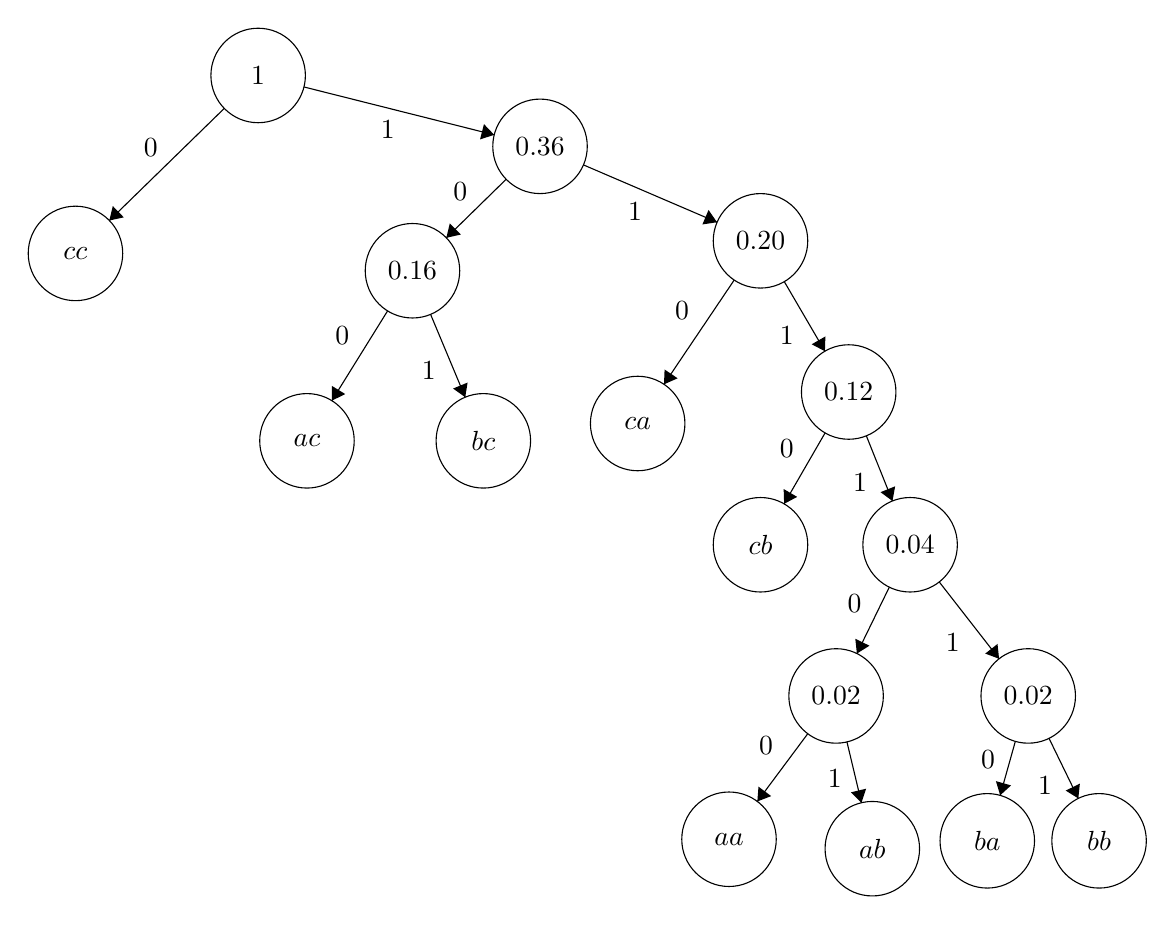
\begin{tikzpicture}[scale=0.2]
\tikzstyle{every node}+=[inner sep=0pt]
\draw [black] (22.6,-5) circle (3);
\draw (22.6,-5) node {$1$};
\draw [black] (11,-16.3) circle (3);
\draw (11,-16.3) node {$cc$};
\draw [black] (40.5,-9.5) circle (3);
\draw (40.5,-9.5) node {$0.36$};
\draw [black] (32.4,-17.4) circle (3);
\draw (32.4,-17.4) node {$0.16$};
\draw [black] (54.5,-15.5) circle (3);
\draw (54.5,-15.5) node {$0.20$};
\draw [black] (25.7,-28.2) circle (3);
\draw (25.7,-28.2) node {$ac$};
\draw [black] (36.9,-28.2) circle (3);
\draw (36.9,-28.2) node {$bc$};
\draw [black] (46.7,-27.1) circle (3);
\draw (46.7,-27.1) node {$ca$};
\draw [black] (60.1,-25.1) circle (3);
\draw (60.1,-25.1) node {$0.12$};
\draw [black] (54.5,-34.8) circle (3);
\draw (54.5,-34.8) node {$cb$};
\draw [black] (64,-34.8) circle (3);
\draw (64,-34.8) node {$0.04$};
\draw [black] (59.3,-44.4) circle (3);
\draw (59.3,-44.4) node {$0.02$};
\draw [black] (71.5,-44.4) circle (3);
\draw (71.5,-44.4) node {$0.02$};
\draw [black] (52.5,-53.5) circle (3);
\draw (52.5,-53.5) node {$aa$};
\draw [black] (61.6,-54.1) circle (3);
\draw (61.6,-54.1) node {$ab$};
\draw [black] (68.9,-53.6) circle (3);
\draw (68.9,-53.6) node {$ba$};
\draw [black] (76,-53.6) circle (3);
\draw (76,-53.6) node {$bb$};
\draw [black] (20.45,-7.09) -- (13.15,-14.21);
\fill [black] (13.15,-14.21) -- (14.07,-14.01) -- (13.37,-13.29);
\draw (15.78,-10.17) node [above] {$0$};
\draw [black] (25.51,-5.73) -- (37.59,-8.77);
\fill [black] (37.59,-8.77) -- (36.94,-8.09) -- (36.69,-9.06);
\draw (30.83,-7.82) node [below] {$1$};
\draw [black] (38.35,-11.59) -- (34.55,-15.31);
\fill [black] (34.55,-15.31) -- (35.47,-15.1) -- (34.77,-14.39);
\draw (35.43,-12.97) node [above] {$0$};
\draw [black] (43.26,-10.68) -- (51.74,-14.32);
\fill [black] (51.74,-14.32) -- (51.2,-13.54) -- (50.81,-14.46);
\draw (46.53,-13.01) node [below] {$1$};
\draw [black] (30.82,-19.95) -- (27.28,-25.65);
\fill [black] (27.28,-25.65) -- (28.13,-25.23) -- (27.28,-24.71);
\draw (28.42,-21.51) node [left] {$0$};
\draw [black] (33.55,-20.17) -- (35.75,-25.43);
\fill [black] (35.75,-25.43) -- (35.9,-24.5) -- (34.98,-24.88);
\draw (33.91,-23.73) node [left] {$1$};
\draw [black] (52.83,-17.99) -- (48.37,-24.61);
\fill [black] (48.37,-24.61) -- (49.24,-24.23) -- (48.41,-23.67);
\draw (49.99,-19.96) node [left] {$0$};
\draw [black] (56.01,-18.09) -- (58.59,-22.51);
\fill [black] (58.59,-22.51) -- (58.62,-21.57) -- (57.75,-22.07);
\draw (56.65,-21.54) node [left] {$1$};
\draw [black] (58.6,-27.7) -- (56,-32.2);
\fill [black] (56,-32.2) -- (56.83,-31.76) -- (55.97,-31.26);
\draw (56.65,-28.72) node [left] {$0$};
\draw [black] (61.22,-27.88) -- (62.88,-32.02);
\fill [black] (62.88,-32.02) -- (63.05,-31.09) -- (62.12,-31.46);
\draw (61.3,-30.84) node [left] {$1$};
\draw [black] (62.68,-37.49) -- (60.62,-41.71);
\fill [black] (60.62,-41.71) -- (61.42,-41.21) -- (60.52,-40.77);
\draw (60.95,-38.51) node [left] {$0$};
\draw [black] (65.85,-37.16) -- (69.65,-42.04);
\fill [black] (69.65,-42.04) -- (69.55,-41.1) -- (68.77,-41.71);
\draw (67.18,-41.01) node [left] {$1$};
\draw [black] (57.5,-46.8) -- (54.3,-51.1);
\fill [black] (54.3,-51.1) -- (55.18,-50.76) -- (54.37,-50.16);
\draw (55.32,-47.55) node [left] {$0$};
\draw [black] (59.99,-47.32) -- (60.91,-51.18);
\fill [black] (60.91,-51.18) -- (61.21,-50.29) -- (60.24,-50.52);
\draw (59.69,-49.67) node [left] {$1$};
\draw [black] (70.68,-47.29) -- (69.72,-50.71);
\fill [black] (69.72,-50.71) -- (70.41,-50.08) -- (69.45,-49.81);
\draw (69.43,-48.45) node [left] {$0$};
\draw [black] (72.82,-47.09) -- (74.68,-50.91);
\fill [black] (74.68,-50.91) -- (74.78,-49.97) -- (73.88,-50.41);
\draw (73.05,-50.09) node [left] {$1$};
\end{tikzpicture}
\end{center}

$$n_{sr} = 2.16$$

Poruka:

$$111110100101111111111111111100111101$$

Po svim stanjima: $n_{sr} = 0.145 \cdot 3.18 + 0.161 \cdot 3 + 0.693 \dot 2.16 = 2.44098$

$$\overline{I(X)} = \frac{0.90667}{\tau}$$

Iskorištenost: 90.60\%
\newpage
\section*{Zadatak 8\label{Z8}}

\underline{Postavka:}

Neki binarni kanal veze sa šumom prenosi dva simbola 0 i 1, pri čemu su vjerovatnoće greške nule i jedinice 0.2 i 0.2 respektivno. Odredite količinu prenesene informacije kroz ovaj kanal ukoliko vjerovatnoća pojave nule na ulazu u kanal iznosi 0.8, te odredite njegov kapacitet.

\underline{Rješenje:}\\

Vjerovatnoća pojave jedinice na ulazu je dakle 0.2.

Ulazni simboli: $y_1 = 0$ i $y_2 = 1$

Izlazni simboli: $z_1 = 0$ i $z_2 = 1$

Iz postave zadatka zaključujemo sljedeće:

$$p(z_1/y_1) = 0.8$$
$$p(z_2/y_1) = 0.2$$
$$p(z_1/y_2) = 0.2$$
$$p(z_2/y_2) = 0.8$$
$$p(y_1) = 0.8$$
$$p(y_2) = 0.2$$

Prema teoremi o totalnoj vjerovatnoći, vjerovatnoće simbola na izlazu su:

$$p(z_1) = p(y_1) p(z_1 / y_1) + p(y_2) p(z_1 / y_2) = 0.68$$
$$p(z_2) = 1 - p(z_1) = 0.32$$

Entropije ulaznih i izlaznih simbola:

$$H(Y) = - \frac{1}{\ln{2}} ( p(y_1) \ln{p(y_1)} +  p(y_2) \ln{p(y_2)}) \approx 0.721$$
$$H(Z) \approx 0.904$$

Potrebne su nam "djelimično" uvjetne entropije:

$$H(Z/y_1) = - \frac{1}{\ln{2}} ( p(z_1/y_1) \ln{p(z_1/y_1)} + p(z_2 / y_1) \ln{p(z_2 / y_1)}) \approx 0.721$$
$$H(Z/y_2) \approx 0.721$$

Dakle $$H(Z/y_1) = H(Z/y_2)$$

Pa je uvjetna entropija:

$$H(Z/Y) = p(y_1) H(Z/y_1) + p(y_2) H(Z/y_2) \approx 0.721$$

Prosječna prenesena količina informacije kroz kanal:

$$I(Y, Z) = H(Z) - H(Z / Y) \approx 0.183$$

Kapacitet kanala veze:

$$C_c = max \overline{I(\eta, \zeta)} \approx \frac{0.2796}{\tau}$$

Kapacitet ovog kanala je 27.96\% kapaciteta koji bi imao odgovarajući kanal bez šuma.

\newpage
\section*{Zadatak 9\label{Z9}}

\underline{Postavka:}

Izvor informacija bez memorije emitira dvije poruke a i b, pri čemu vjerovatnoća emitiranja poruke a iznosi p(a) = 0.8. Ove poruke se zatim kodiraju, i prenose kroz binarni kanal veze sa šumom koji koristi dva simbola 0 i 1, pri čemu su vjerovatnoće greške nule i jedinice 0.25 i 0.05 respektivno. Odredite količinu prenesene informacije kroz komunikacioni kanal, brzinu prenosa informacija kroz komunikacioni kanal, procenat iskorištenja kanala veze i vjerovatnoću greške u prenosu ukoliko se koristi

a)Prosto kodiranje a → 0 i b → 1 uz dekodiranje zasnovano na klasifikaciji Sa = {0} i Sb = {1};

b)Zaštitno kodiranje a → 000 i b → 111 uz dekodiranje zasnovano na klasifikaciji Sa = {000, 001, 010, 100} i Sb = {011, 101, 110, 111}.

\underline{Rješenje:}\\

a)\\

$$x_1 = a; p(a) = p(x_1) = 0.8$$
$$x_2 = b; p(b) = p(x_2) = 0.2$$

Ulazni simboli: $y_1 = 0$ i $y_2 = 1$

Izlazni simboli: $z_1 = 0$ i $z_2 = 1$

Iz postave zadatka zaključujemo sljedeće:

$$p(0/x_1) = p(z_1/y_1) = 0.75$$
$$p(1/x_1) = p(z_2/y_1) = 0.25$$
$$p(0/x_2) = p(z_1/y_2) = 0.05$$
$$p(1/x_2) = p(z_2/y_2) = 0.95$$

$$p(w_1) = p(x_1) p(0/x_1) + p(x_2) p(0/x_2) = 0.61 = p(0)$$
$$p(w_2) = 0.39 = p(1)$$

Entropija i uslovna entropija:

$$H(W) = - \frac{1}{\ln{2}} ( p(w_1) ln p(w_1) + p(w_2) ln p(w_2) ) = 0.9648$$

$$H(W/x_1) = 0.811$$
$$H(W/x_2) = 0.286$$

$$H(W/X) = p(x_1) H(W/x_1) + p(x_2) H(W / x_2) = 0.8 \cdot 0.811 + 0.2 \cdot 0.286 = 0.706$$ 

$$I(X, W) = H(W) - H(W / X) = 0.9648 - 0.706 = 0.2588$$

Vjerovatnoća greške je $p_e = 1 - p(a) \cdot p(0 / x_1) - p(b) \cdot p(1 / x_2) = 0.21$\\

Brzina prenosa je: $\overline{I(X, W)} = \frac{I(X, W)}{T_{sr}} = \frac{0.3328}{T_{sr}}$\\

\newpage
b)\\

$$w_1 = S_a$$
$$w_2 = S_b$$

Ulazni simboli: $y_1 = 0$ i $y_2 = 1$

Izlazni simboli: $z_1 = 0$ i $z_2 = 1$

$$x_1 = a; p(a) = p(x_1) = 0.8...x_1 \to y_1y_1y_1$$
$$x_2 = b; p(b) = p(x_2) = 0.2...x_2 \to y_2y_2y_2$$

$$S_a = {z_1z_1z_1, z_1z_1z_2, z_1z_2z_1, z_2z_1z_1}$$
$$S_b = {z_1z_2z_2, z_2z_1z_2, z_2z_2z_1, z_2z_2z_2}$$

$$p(w_1 / x_1) = p(z_1z_1z_1 / y_1y_1y_1) + p(z_1z_1z_2 / y_1y_1y_1) + p(z_1z_2z_1 / y_1y_1y_1) + p(z_2z_1z_1 / y_1y_1y_1)$$
$$p(w_1 / x_1) = p(z_1 / y_1)^3 + 3 p(z_1 / y_1)^2 p(z_2 / y_1) = 0.84375$$
$$p(w_2 / x_1) = 1 - 0.84375 = 0.15625$$
$$p(w_1 / x_2) = 0.00725$$
$$p(w_2 / x_2) = 0.99275$$

$$p(w_1) = p(x_1) p(w_1 / x_1) + p(x_2) p(w_1 / x_2) = 0.67645$$
$$p(w_2) = 0.32355$$

$$H(W) = - \frac{1}{\ln{2}} ( p(w_1) \ln p(w_1) + p(w_2) \ln p(w_2) ) = 0.9082$$
$$H(W / x_1) = 0.625262$$
$$H(W / x_2) = 0.06195$$

$$H(W / X) = p(x_1) H(W / x_1) + p(x_2) H( W / x_2) = 0.5125$$

$$I(X, W) = H(W) - H(W / X) = 0.3956$$

Vjerovatnoća greške:
$$p_e = 1 - 0.8 \cdot 0.84375 - 0.2 \cdot 0.99275 = 0.126$$
 
Brzina prenosa:

$$\overline{I(X, W)} = \frac{0.1318}{\tau}$$


\end{document}